\documentclass[10pt,twoside,openright]{article}

%---------------------------------------------------------------------------
%List of packages with theid respective use, you can uncomment if not used
%---------------------------------------------------------------------------

%--------------layout of the document--------------
% this package is used to get a wider A4 paper
\usepackage{a4wide}
% these packages are used to produce nicer captions
\usepackage[font={small},labelfont={bf,sf},width=0.8\textwidth, singlelinecheck=false]{caption}
%\usepackage[font={small},labelfont={bf,sf},hang,singlelinecheck=false]{caption}
% use the titlesec package to change the section 
\usepackage[calcwidth,newparttoc]{titlesec}
% use the titletoc package to change the toc
\usepackage{titletoc}
% hyperrefs used in the produced pdf file
\usepackage[a4paper,plainpages=false]{hyperref}
% this package is used for colored text
\usepackage{xcolor}
%\usepackage[cmyk]{xcolor}
% this package is used for intelligent spaces
\usepackage{xspace}
% this package is a collection of fonts of symbols and characters that aren't always included in standard distributions of TeX
\usepackage{amsfonts}
% this package defines the full set of symbol names for two fonts of extra symbols included in the amsfonts collection
\usepackage{amssymb}
% this package is used to create custom headers and footers
\usepackage{fancyhdr}
\pagestyle{fancy}
% this package used to produce a different style of page numbering
% \usepackage[auto]{chappg}
% this package allows you to have toc's for each chapter
% \usepackage{minitoc}
% package used to make an index
% \usepackage{makeidx} 
% use this package to use times new roman fonts
% \usepackage{times}
% use this package for striketrough fonts
%\usepackage[normalem]{ulem}
\usepackage{lmodern}
\usepackage{rotating}
\usepackage[T1]{fontenc}
%--------------figure and table adaptations--------------
% this package is used for figures with are spread over two or more pages
\usepackage{captcont}
% this package is used for creating table with multirows
\usepackage{multirow}
% this package enables one to put several figures next to each other
\usepackage{subfigure}
%Show floats (images, tables, ?) only AFTER they have been referenced for the first time:
\usepackage{flafter} 
% enables footnotes in a table itself
\usepackage{threeparttable}
% Publication quality tables 
\usepackage{booktabs}  % http://archive.cs.uu.nl/mirror/CTAN/macros/latex/contrib/booktabs/booktabs.pdf
% needed to change rowheight in tables
\usepackage{array}
%figuren opnemen en eps toelaten
\usepackage{graphicx}
%figuren opnemen en eps toelaten
\usepackage{graphicx}
\usepackage{epstopdf}
% this package is the natural frontend for pgf (a package for creating graphics in an inline manner).
%\usepackage{tikz}
%\usetikzlibrary{arrows,shapes,calendar,matrix,backgrounds,folding}
% this package is used to wrap text around figures
% \usepackage{wrapfig}
% \usepackage{floatflt}

%--------------mathematical stuff--------------
% this package enhances the typeset appearance of mathematical formulas
\usepackage{amsmath}
% this package provides access to bold math symbols
\usepackage{bm}
% extra symbols available: http://home.online.no/~pjacklam/latex/textcomp.pdf
\usepackage{textcomp}
% larger integrals to adapt to specific use
\usepackage{bigints}
% use this package to use the garamond font
% \usepackage[garamond]{mathdesign}
% this package is used to create partitioned matrices
%\usepackage{pmat}
% nice fractions a/b
\usepackage{nicefrac}

%--------------Interesting environments style--------------
% these packages provides an environment for algorithms (cfr. Pseudocode)
\usepackage[ruled]{algorithm2e} % info: http://archive.cs.uu.nl/mirror/CTAN/macros/latex/contrib/algorithm2e/doc/algorithm2e.pdf
%\usepackage{algorithm}  
%\usepackage{algorithmic}
% The thmtools bundle is a collection of packages that is designed to provide an easier interface to theorems
%\usepackage{thmtools}
% use this package for url's
\usepackage{url}
% this package is used to get nicer chemical notations
%\usepackage[version=3]{mhchem}
% create todo notes to show where what needs adaptation
\usepackage[colorinlistoftodos, textwidth=4cm, shadow]{todonotes}

%--------------bibliograhy stuff--------------
% this package is used to produce both author-date and standard numerical citations for BibTeX bibliographies
\usepackage[square,numbers]{natbib}
%round

%--------------Others--------------
% this package allows you to resume a previous enumerate environment
\usepackage{enumitem}
% this package is used to generate lipsum code
\usepackage{lipsum}
% this package is used for if then environments
\usepackage{ifthen}
%All text, within the landscape environment is rotated through 90 degrees:
\usepackage{lscape}
% this package is used to rotate text
% \usepackage{rotating}
\usepackage{pgfplots}
\usepackage{svg}
%---------------------------------------------------------------------------
% Some adaptations and settings of the distances in document
%---------------------------------------------------------------------------
% set interline set to ...
\renewcommand{\baselinestretch}{1.2}
% space between two paragraphs should be larger than between two lines of text
\newcommand{\npar} {\par \vspace{2.3ex plus 0.3ex minus 0.3ex}} 
% no indentations
\setlength{\parindent}{0cm}
% makes all pages the height of the text on that page, and no extra vertical space is added
\raggedbottom


%%%%%%%%%%%% voor procesdiagrammen %%%%%%%%%%%%
\usepackage{tikz}
\usetikzlibrary{arrows,positioning}
\usetikzlibrary{shapes,arrows}

\tikzstyle{block} = [draw, fill=white, rectangle, 
minimum height=3.5em, minimum width=3.5em]
\tikzstyle{input} = [coordinate]
\tikzstyle{output} = [coordinate]
\tikzstyle{leeg} = [coordinate]
\tikzstyle{pinstyle} = [pin edge={to-,thin,black}]
\tikzstyle{triangle} = [draw, fill=white, regular polygon, regular polygon sides=3,shape border rotate=90]
\tikzset{sum/.style n args = {4}{draw, circle, node distance = 2cm, minimum size=5mm, alias=sum,
		append after command={
			node at (sum.north) [port, below=1pt] {$#1$}
			node at (sum.west) [port, right=1pt] {$#2$}
			node at (sum.south) [port, above=1pt] {$#3$}
			node at (sum.east) [port, left=1pt] {$#4$}
		},
}}

%---------------------------------------------------------------------------
% making glossary of abbrevitations and symbols
% ATTENTION: To make the glossaries working, you need to adapt your output
% profiles of the editor you're working in (KIle, Texniccenter)
% See http://biomath.ugent.be/wiki/index.php/Software#Glossaries for
% Explanation.
% If you're not able to make it work, consider using the nomenclature package, also given above
%---------------------------------------------------------------------------
\usepackage[toc,acronym,shortcuts,nonumberlist]{glossaries}
\makeglossaries
\makeindex

% this package is used to create a nomenclature list (alternative to the glossaries package; easier, but less powerfull)
%\usepackage[noprefix]{nomencl}
% this package is used to create a list of symbols (alternative to the glossaries package; easier, but less powerfull)
% \usepackage[final,pageno]{listofsymbols}

%---------------------------------------------------------------------------
%code visualization of code snippets + characteristics; done with listings
%can be used for multiple code languages, but is different from pseudocode
%---------------------------------------------------------------------------

\definecolor{mygreen}{rgb}{0,0.6,0}
\definecolor{lightgray}{gray}{0.90}
\usepackage{listings}
\lstdefinestyle{matlab}{
	language=Matlab,                % choose the language of the code
	basicstyle=\footnotesize\ttfamily,       % the size of the fonts that are used for the code
	numbers=none,                   % where to put the line-numbers
	numberstyle=\scriptsize,      % the size of the fonts that are used for the line-numbers
	stepnumber=1,                   % the step between two line-numbers. If it is 1 each line will be numbered
	numbersep=5pt,                  % how far the line-numbers are from the code
	backgroundcolor=\color{lightgray},  % choose the background color. You must add \usepackage{color}
	showspaces=false,               % show spaces adding particular underscores
	showstringspaces=false,         % underline spaces within strings
	showtabs=false,                 % show tabs within strings adding particular underscores
	frame=none,           % adds a frame around the code
	tabsize=2,          % sets default tabsize to 2 spaces
	captionpos=b,           % sets the caption-position to bottom
	breaklines=true,        % sets automatic line breaking
	breakatwhitespace=false,    % sets if automatic breaks should only happen at whitespace
	xleftmargin=15pt,
	xrightmargin=5pt,
	commentstyle=\color{mygreen},    %teal => gray for printing
	keywordstyle=\color{blue},
	stringstyle=\color{orange},
	escapeinside={\%*}{*}            % if you want to add LaTeX within your code}
}


\definecolor{identifiercolor}{rgb}{0.15,0.15,0.5} %{.4,.6,.56}
\definecolor{stringcolor}{gray}{0.5}
\definecolor{inactivecolor}{rgb}{0,0,0}
\definecolor{commentcolor}{rgb}{0,0.6,0.5}
\lstdefinestyle{mathematica}{
	language=Mathematica,
	basicstyle={\footnotesize\def\fvm@Scale{.85}\fontfamily{fvm}\selectfont},
  	breaklines=true,
  	escapeinside={\%*}{*)},
  	commentstyle={\color{commentcolor}},
  	keywordstyle={\bfseries\color{inactivecolor}},
  	stringstyle={\bfseries\color{stringcolor}},
  	identifierstyle={\bfseries\color{identifiercolor}},
  	otherkeywords={DiscretizeRegion},
  	showstringspaces=false,
  	backgroundcolor=\color{lightgray},
  	xleftmargin=15pt,
	xrightmargin=5pt,
  }


%---------------------------------------------------------------------------
% new command to make superscripts in the text/tables mode
%---------------------------------------------------------------------------
%http://anthony.liekens.net/index.php/LaTeX/SubscriptAndSuperscriptInTextMode
\newcommand{\superscript}[1]{\ensuremath{^{\textrm{#1}}}} 
\newcommand{\subscript}[1]{\ensuremath{_{\textrm{#1}}}}
% new commands to create nicer sub and superscripts in math mode
\newcommand{\sms}[1]{\mbox{\tiny{#1}}}
\newcommand{\lss}[1]{_{\mbox{\tiny{#1}}}}
\newcommand{\uss}[1]{^{\mbox{\tiny{#1}}}}

%---------------------------------------------------------------------------
% Short version commando to introduce figures. 
%---------------------------------------------------------------------------
%\mijnfiguur[H]{width=5cm}{bestandsnaam}{Het bijschrift bij deze figuur}{label}
\newcommand{\mijnfiguur}[5][ht]{            % Het eerste argument is standaar `ht'.
    \begin{figure}[#1]                      % Beginnen van de figure omgeving
        \begin{center}                      % Beginnen van de center omgeving
            \includegraphics[#2]{#3}        % Het eigenlijk invoegen van de figuur (2: opties, 3: bestandsnaam)
        \end{center}
        \caption{#4\label{#5}}          % Het bijschrift (argument 4) en het label (argument 3)
    \end{figure}
    }

%-----------------------------------------------------------------------------------------
% PDF properties (you only see this as document properties (metadata) of your pdf-document
%-----------------------------------------------------------------------------------------
\hypersetup{
    pdfauthor = {Your name},
    pdftitle = {Your title},
    pdfkeywords = {some relevant keywords}}

\setcounter{MaxMatrixCols}{20}

\usepackage{tcolorbox}
\usepackage{lipsum}
\usepackage{verbatim}

%path to graphics
\graphicspath{{fig/}}


%-------------------------------
% Opgave / Oplossing environment
%-------------------------------

\usepackage[framemethod=TikZ]{mdframed}
\mdfdefinestyle{warning}{%
	linecolor=white,
	align=center,
	roundcorner=3pt,
	innertopmargin=6pt,
	innerbottommargin=5pt,
	innerrightmargin=10pt,
	innerleftmargin=10pt,
	backgroundcolor=black!12,
	skipabove=0.4\baselineskip
}

\newcounter{opgave}[section]\setcounter{opgave}{0}
\renewcommand{\theopgave}{\arabic{section}.\arabic{opgave}}
\newenvironment{opgave}[2][]{%
	\refstepcounter{opgave}
	\label{#2}
	\mdfsetup{%
		frametitle={%
			\tikz[baseline=(current bounding box.east),outer sep=0pt]
			\node[anchor=east,rectangle,fill=gray!40]
			{\strut Exercise~\theopgave:~#1};}%
	}
	\mdfsetup{%
		innertopmargin=10pt,linecolor=white!30,%
		linewidth=0pt,topline=true,%
		frametitleaboveskip=\dimexpr-\ht\strutbox\relax%
	}

	\begin{mdframed}[]\relax}{%
\end{mdframed}}


\newenvironment{oplossing}[2][]{%
	\mdfsetup{%
		frametitle={%
			\tikz[baseline=(current bounding box.east),outer sep=0pt]
			\node[anchor=east,rectangle,fill=gray!20]
			{\strut Solution};}%
	}
	\mdfsetup{%
		innertopmargin=10pt,linecolor=white!30,
		linewidth=0pt,topline=true,%
		frametitleaboveskip=\dimexpr-\ht\strutbox\relax%
	}
	
	\begin{mdframed}[]\relax}{%
\end{mdframed}}

% ------------------
% Leeg vak
% ------------------

\newlength{\lvaklength}

\newcommand{\leegvak}[2]{\noindent\framebox[#1]{\parbox{#1}{\vspace{#2}}}}
\newcommand{\leegvakf}[1]{
\setlength{\lvaklength}{0cm}
\addtolength{\lvaklength}{0.925\textwidth}
%\addtolength{\lvaklength}{-\leftmargin}
\leegvak{\lvaklength}{#1}
}

\newcommand{\leegvakg}[1]{
\setlength{\lvaklength}{0cm}
\addtolength{\lvaklength}{0.875\textwidth}
%\addtolength{\lvaklength}{-\leftmargin}
\leegvak{\lvaklength}{#1}
}

\newcommand{\solbox}[2]{
\noindent\framebox[0.925\textwidth]{
\parbox{#1}{\vspace{#1}}
\begin{minipage}[c][#1][c]{0.925\textwidth}
	\centering
	#2
\end{minipage}
}}

%---------------------------------------------------------------------------
%---------------------------------------------------------------------------
% The actual document starts here
%---------------------------------------------------------------------------
%---------------------------------------------------------------------------
\begin{document}

\title{%
  Control Theory Hands-on Practical \\
  \Large Hovering a table tennis ball at a fixed height}
  
\author{Dr.~Tijs W. Alleman$^{1,*}$, Daniel Illana$^{1}$, Dr.~Gauthier Vanhaelewyn$^{1}$}
\maketitle

$^*$Corresponding author: \url{tijs.alleman@ugent.be} \\
$^1$BIOMATH, Department of Data Analysis and Mathematical Modelling, Ghent University, Coupure Links 653, Ghent, 9000, Belgium\\
Available on GitHub: \url{https://github.com/twallema/hovering-table-tennis-ball}\\

\begin{center}
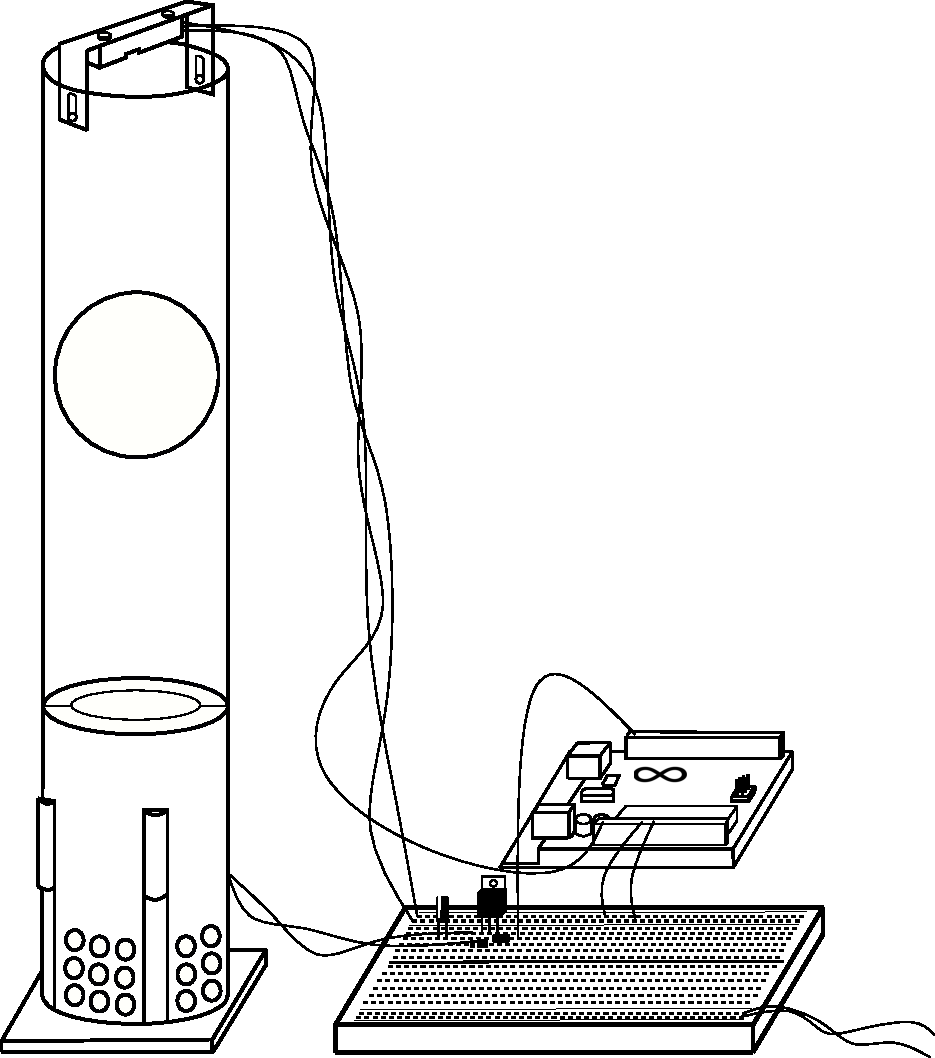
\includegraphics[width=5cm]{setup.pdf}
\end{center}

\paragraph{Aim} In this practical, we turn control theory into practice by hovering a table tennis ball at a fixed height in a transparent tube. We use an Arduino Uno to build a closed loop feedback controller. We measure the ball's height using an infrared distance sensor at the top of the tube, which we the use to control a fan at the bottom of the tube. First, we study the setup's open-loop behavior and gather response data to calibrate a mathematical model. We then use Matlab's Simulink environment to perform an in-silico tuning of several closed-loop feedback controllers, such as the Proportional-Integral-Derivative (PID) controller and Linear-Quadratic Regulator (LQR) state feedback controller. Finally, the performance of the tuned controllers is examined and compared using the experimental setup. This setup serves as an intuitive and visual test bed for the closed-loop feedback controllers introduced in the theoretical course. Our aim is to introduce students to the use of electronics, the unfortunate reality of noisy sensors and dead time, along with their implications on closed-loop stability, the application of control theory to non-linear systems, and to the use of mathematical modeling to support the in-silico design of a suitable controller.


\setcounter{tocdepth}{2}
\tableofcontents

\clearpage
\section{Introduction}

\subsection{Electronics}

To build the practical setup, we first need to familiarise ourselves with the bread and butter of electronics: the resistor, capacitor, diode and transistor. In this short intro we use the hydraulic circuit analogy, to explain some basic concepts. In this analogy, an electrical circuit is thought to be a hydraulic circuit consisting of pipes, valves, pumps, etc. Charge is represented by the water amount, voltage is represented by the water pressure, and current is represented by the water flow.

\paragraph{Resistor}
As the name implies, resistors add resistance to the circuit and reduce the flow of electrical current. In the hydraulical circuit analogy a resistance is represented by a throttling valve, or alternatively, as rocks in a river, hindering the flow of water. Resistors are typically represented as a pointy squiggle with a value next to it (Fig.~\ref{fig:resistor}). In electronic devices, resistors are used to avoid damage resulting from high currents. When building an electronic circuit, it is paramount to check the amount of current flowing through each analog component by using Ohm's law,
\begin{equation}
I = \frac{V}{R},
\label{eqn:Ohms law}
\end{equation}
where V is voltage in Volt (V), I is the electric current in Amps (A) and R is the resistance in Ohms ($\Omega$). Most electronic components, f.i. an LED, have little internal resistance. When applying even the smallest voltage directly to an LED, the LED will light up briefly and then shutdown forever. Generally speaking, overloading electronic circuits by mistake is common and not very dangerous. \textbf{In any case, when noticing the characteristic smell of a shortcircuit (a combination of ozone and burnt plastic) during this practical, please pull out the wall plug immediately!} During this practical we will use a 2.2 $k\Omega$ resistor to limit the current of a voltage sent from the Arduino Uno to a transistor.
\mijnfiguur[h!]{width=6cm}{resistor.jpg}{(upper) real life resistor. (lower) schematic representation of a transistor.}{fig:resistor}

\paragraph{Capacitor}
A capacitor is a component that stores electricity and then discharges it into the circuit when there is a drop in current. You can think of a capacitor as a water storage tank that releases water when there is a drought to ensure a steady stream. Therefore, capacitors are typically used to filter a noisy current. Further, capacitors are preferred over batteries in applications that require a rapid discharge, such as in a defibrillator. The values that you will typically encounter in most capacitors are measured in picofarad (pF), nanofarad (nF), and microfarad ($\mu F$). The most commonly encountered types of capacitors are ceramic disc capacitors that look like tiny M\&Ms with two wires sticking out of them and electrolytic capacitors that look more like small cylindrical tubes with two wires coming out the bottom (Fig.~\ref{fig:capacitor}). The main difference is that ceramic disc capacitors are non-polarized, meaning that electricity can pass through them no matter how they are inserted in the circuit. Opposed, electrolytic capacitors are polarized, meaning one leg needs to be connected to the ground side of the circuit and the other leg must be connected to power. For this practical we will be using a 22 $\mu F$ electrolytic capacitor as an analog filter for the power supply of the IR proximity sensor. \textbf{Because the provided capacitor is electrolytic, please make sure you respect its polarity.}

\mijnfiguur[h!]{width=7cm}{capacitor.jpg}{(left) real life ceramic capacitor and schematic representation (right) real life electrolytic capacitor and schematic representation.}{fig:capacitor}

%bron figuren: https://www.instructables.com/id/Basic-Electronics/

\paragraph{Diode}
A diode only allows electrical current to pass through them in one direction, its hydraulic analogy is a non-return valve. Diodes are useful to prevent electricity from flowing in the wrong direction. When the voltage applied to an electric DC motor is abruptly switched off, the fan will keep spinning for a short while. As such, the motor will act as a generator of current until its blades come to a standstill. Charge will build up on what was the negative terminal of the motor and this charge will want 'a way out'. Adding a diode in parallel with the motor provides a path for dissipation of stored energy when the voltage is cut. Similar to the electrolytic capacitor, the diode is polarised and the ring found on one end of the diode indicates the side of the diode which connects to ground. \textbf{When building the setup, please mind that the ring on the diode points in the right direction (Fig.~\ref{fig:fritzing}).}

\mijnfiguur[h!]{width=6cm}{diode.jpg}{(upper) real life diode (lower) schematic representation of a diode.}{fig:diode}
%\mijnfiguur[h!]{width=5cm}{flybackDiode.png}{The flyback diode allows charge to dissipate without arcing across the switch (analog component), or without flowing back to ground through the +5 V voltage supply.}{fig:flybackDiode}


\paragraph{Transistor} A transistor can act as a switch or gate for electronic signals, opening and closing many times per second. It typically has three pins: the base, emitter and collector pins (Fig.~\ref{fig:transistor}). A transistor uses a small electrical current at its base pin to control the current passing between its collector and emitter pins. The amount of current allowed to pass between the collector and emitter pins is proportional to the voltage being applied at the base pin. A transistor is therefore a good way of controlling a high voltage/high current circuit (fan motor, 12 VDC) using a low voltage/low current signal (Arduino, 5 VDC). An (inperfect) hydraulic analogy for a transistor is an adjustable valve. Passing current through a transistor costs energy and therefore observing a voltage drop of 1 V over a transistor is common. This energy is dissipated in heat so \textbf{transistors heat up to well over 100 \textdegree C under load. Never touch your transistor while operating the setup!}\\

\mijnfiguur[h!]{width=6cm}{BD537.jpg}{BD537 transistor used to control the fan's motor.}{fig:transistor}

%\begin{tcolorbox}[colback=white,colframe=black,title=\textbf{Takeaway lessons}]
%\begin{itemize}
%\itemsep0em 
%\item A limited number of analog components can be arranged to fulfill specific tasks. This is accomplished by designing the circuit so that the right current is provided to the right component.
%\item Analog components can be combined with programmable microcontrollers so that the amount of current flowing through each analog component can vary/be controlled. This allows to build more complex/interactive electronics.
%\end{itemize}
%\end{tcolorbox}

%bron: https://www.arduino.cc/en/guide/introduction, Arduino voor Dummies (John Nussey)

\subsection{The Arduino Uno Rev 3, its components and signals}

Using only resistors, capacitors, diodes and transistors, it is possible to build simple electronic devices that do a specific job, such as an egg timer or a security buzzer that goes off when you keep the fridge open too long. The behavior of such circuits is solely based on the chemical properties of the components, which need to be computed beforehand to make sure that the right amount of current is flowing through the right components. This makes these simple devices very good at their specific job, but they're limited in what they can do. The microcontroller, a tiny computer present on the Arduino Uno can be used can be used in conjunction with the aforementioned analog circuitry to allow for more advanced behavior. The amount of current flowing through the analog components is now variable and controlled, rather than constant and computed beforehand.\\

Arduino is an open-source electronics platform based on easy-to-use hardware and software. The Arduino hardware consists of a small circuit board containing a microcontroller chip and several connections (Fig.~\ref{fig:ARDUINO_UNO}), allowing us to read inputs such as light on a sensor, a finger on a button, or even a Twitter message - and turn them into an output - activating a motor, turning on an LED, publishing something online. This is accomplished by telling your board what to do when certain inputs are encountered by sending a set of instructions to the microcontroller on the board. To do so you can use the Arduino Software (IDE), as well as other programming languages such as Python and Matlab. In this practical, we'll program our Arduino Uno using the Matlab's Simulink environment. Let's examine the Arduino's components closer.

\paragraph{Microcontroller} You can think of the microcontroller chip itself as the \textit{brains} of the board. The chip used in the Arduino Uno is the ATmega328p, made by Atmel. It’s the large, black component in the center of the board. It’s actually not alone but rather sits in a socket. If you were to remove the microcontroller, it would look like the one shown in Figure \ref{fig:ATmega328p}.

\mijnfiguur[h!]{width=6cm}{ATmega328.jpg}{The brain of the Arduino Uno R3: the Atmel ATmega328p microcontroller.}{fig:ATmega328p}

\paragraph{Header sockets}
The microcontroller socket connects all 28 legs of the ATmega328 microcontroller chip to other sockets, referred to as header sockets, which have been arranged around the board and labeled for ease of use. They are the black sockets that go around the edge of the Arduino board. These are divided up into three main groups: digital pins, analog input pins, and power pins.  All these pins transfer a voltage, which can either be sent as output or
received as an input. These pins are important as they allow additional circuitry to be connected to the board quickly and easily.

\paragraph{Power pins} You use the power pins to distribute power to inputs and outputs wherever it’s needed (Fig.~\ref{fig:ARDUINO_UNO}). GND marks the ground pins, which are essential to complete circuits. There is also a third ground by pin 13. All these pins are linked and share the same \textit{common} ground. You can use the 5V and 3.3V pins to supply power to components or circuits. However, the Arduino can only supply about 40 mA of current without getting damaged. This is enough to power most sensors but not enough to power a larger motor. We'll thus have to supply the power for the blower fan externally.

\paragraph{Digital pins} Signals are defined as time-varying \textit{quantities} conveying information, typically a voltage. So when we talk about signals, just think of them as a voltage that's changing over time. You use the \textit{digital pins}, which run across the top of the board (Fig.~\ref{fig:ARDUINO_UNO}), to \textbf{send and receive} digital signals. Digital signals are made up of a sequence of \textit{bits}. A bit represents only one of two states: off or on, 0 or 1, or in electrical terms, 0V or 5V, but no values in between. The amount of information conveyed by a digital signal is characterised by its number of bits. On the Arduino Uno, a digital signal has 10 bits, giving rise to a total of 1024 possible outcomes, corresponding to a number between 0 and 1023. A temporal graph of a digital signal looks like a series of square waves (Fig.~\ref{fig:signals}). In practice, ten bits means the Arduino Uno and your computer are communicating by sending out ten equally long pulses of 0V or 5V within a set time interval. F.i. the computer will send the Arduino Uno a sequence of 10 bits (zeros or ones) in 1 millisecond, implying each bit is 0.100 milliseconds in length. Then there may be a small pause, say 1 millisecond, after which the Arduino Uno gets 1 millisecond to send the computer ten zeros or ones. These timings typically obey a certain protocol, used globally, such as HDMI and USB serial.

\paragraph{Analog pins} These pins are used to \textbf{receive} analog signals (Fig.~\ref{fig:ARDUINO_UNO}). The fundamental difference between an analog signal and a digital signal is that an analog signal is continuous and can assume all values between 0V or 5V (Fig.~\ref{fig:signals}). However, when receiving a voltage between 0 V and 5 V at pin A0-A5, the voltage is automatically converted to a digital value by the Arduino's on-board analog-to-digital converter before it is sent to your computer. \textbf{Therefore, both analog and digital inputs are represented by a number between 0 and 1023 on your computer, and therefore the maximum resolution of any signal on an Arduino Uno is 1/1024}.

\mijnfiguur[h!]{width=9cm}{analog_digital_signal.pdf}{The fundamental difference between an analog and a digital signal. A continuous analog signal (left). A discrete 6-bit digital signal (right).}{fig:signals}

\paragraph{Pulse Width Modulation}
The very shrewd ones among you may have noticed that there seem to be \textbf{no pins for analog outputs}. In fact, there are, but they’re hidden among the digital pins marked as PWM using the “\textasciitilde” symbol. PWM stands for \textit{Pulse Width Modulation}, which is a technique you can use to mimic a continuous analog output using a discrete digital output. A digital output is either on or off but this can be done extremely quickly. If the output is on half the time and off half the time, it is described as having a 50 percent \textit{duty cycle}. Because it is blinking faster than the human eye can perceive, an LED pulsed using a 50 percent duty cycle looks as though it is at half brightness (Fig.~\ref{fig:PWM}). With a DC motor as an output, a 50 percent duty cycle has the effect of moving the motor at half speed. So in this case PWM allows you to control the speed of a motor by pulsing it at an extremely fast rate. PWM works best for devices with sufficient inertia such as electric motors and pumps.

\mijnfiguur[h!]{width=\textwidth}{PWM.pdf}{From left to right: A 20 \%, 70 \% and 90 \% PWM duty cycle.}{fig:PWM}

\mijnfiguur[h!]{width=16cm}{ARDUINO_UNO.png}{An actual Arduino Uno R3 (left) and a schematic highlighting the most important parts (right).}{fig:ARDUINO_UNO}

%\newpage
%\phantom{hello}

%\begin{tcolorbox}[colback=white,colframe=black,title=\textbf{Takeaway lessons}]
%\begin{itemize}
%\itemsep0em 
%\item A signal is a voltage changing over time.
%\item Analog signals are continuous and can assume any voltage between 0 V and 5 V on the Arduino Uno.
%\item Digital signals are discrete and can only assume 0 V or 5 V, corresponding to zeros and ones. Digital signals are characterised by their number of bits and protocols such as USB serial are needed to allow efficient communication.
%\item Analog signals can be mimicked using a digital signal and this is called \textit{Pulse Width Modulation}.
%\end{itemize}
%\end{tcolorbox}

\section{Practical setup}

\subsection{Materials}

\begin{itemize}
\itemsep0em 
\item Arduino Uno R3
\item Male-male jumper wires
\item Solderless breadboard
\item Sharp 2Y0A21 IR proximity sensor
\item 2.2 $\text{k}\Omega$ resistor
\item BD139 or BD537 transistor
\item Diode
\item 22 $\mu\text{F}$ electrolytic capacitor
\item Sunon 40x40x10 mm 5~VDC blower fan
\item Fan stand, obtained from \url{https://www.instructables.com/Float-a-Ping-Pong-Ball-at-Will}
\item 12~ VDC power supply
\item Transparent polycarbonate tube, 65 cm long
\item USB-A to USB-B cable
\item Table tennis ball
\end{itemize}

\begin{figure}[h!]
\centering
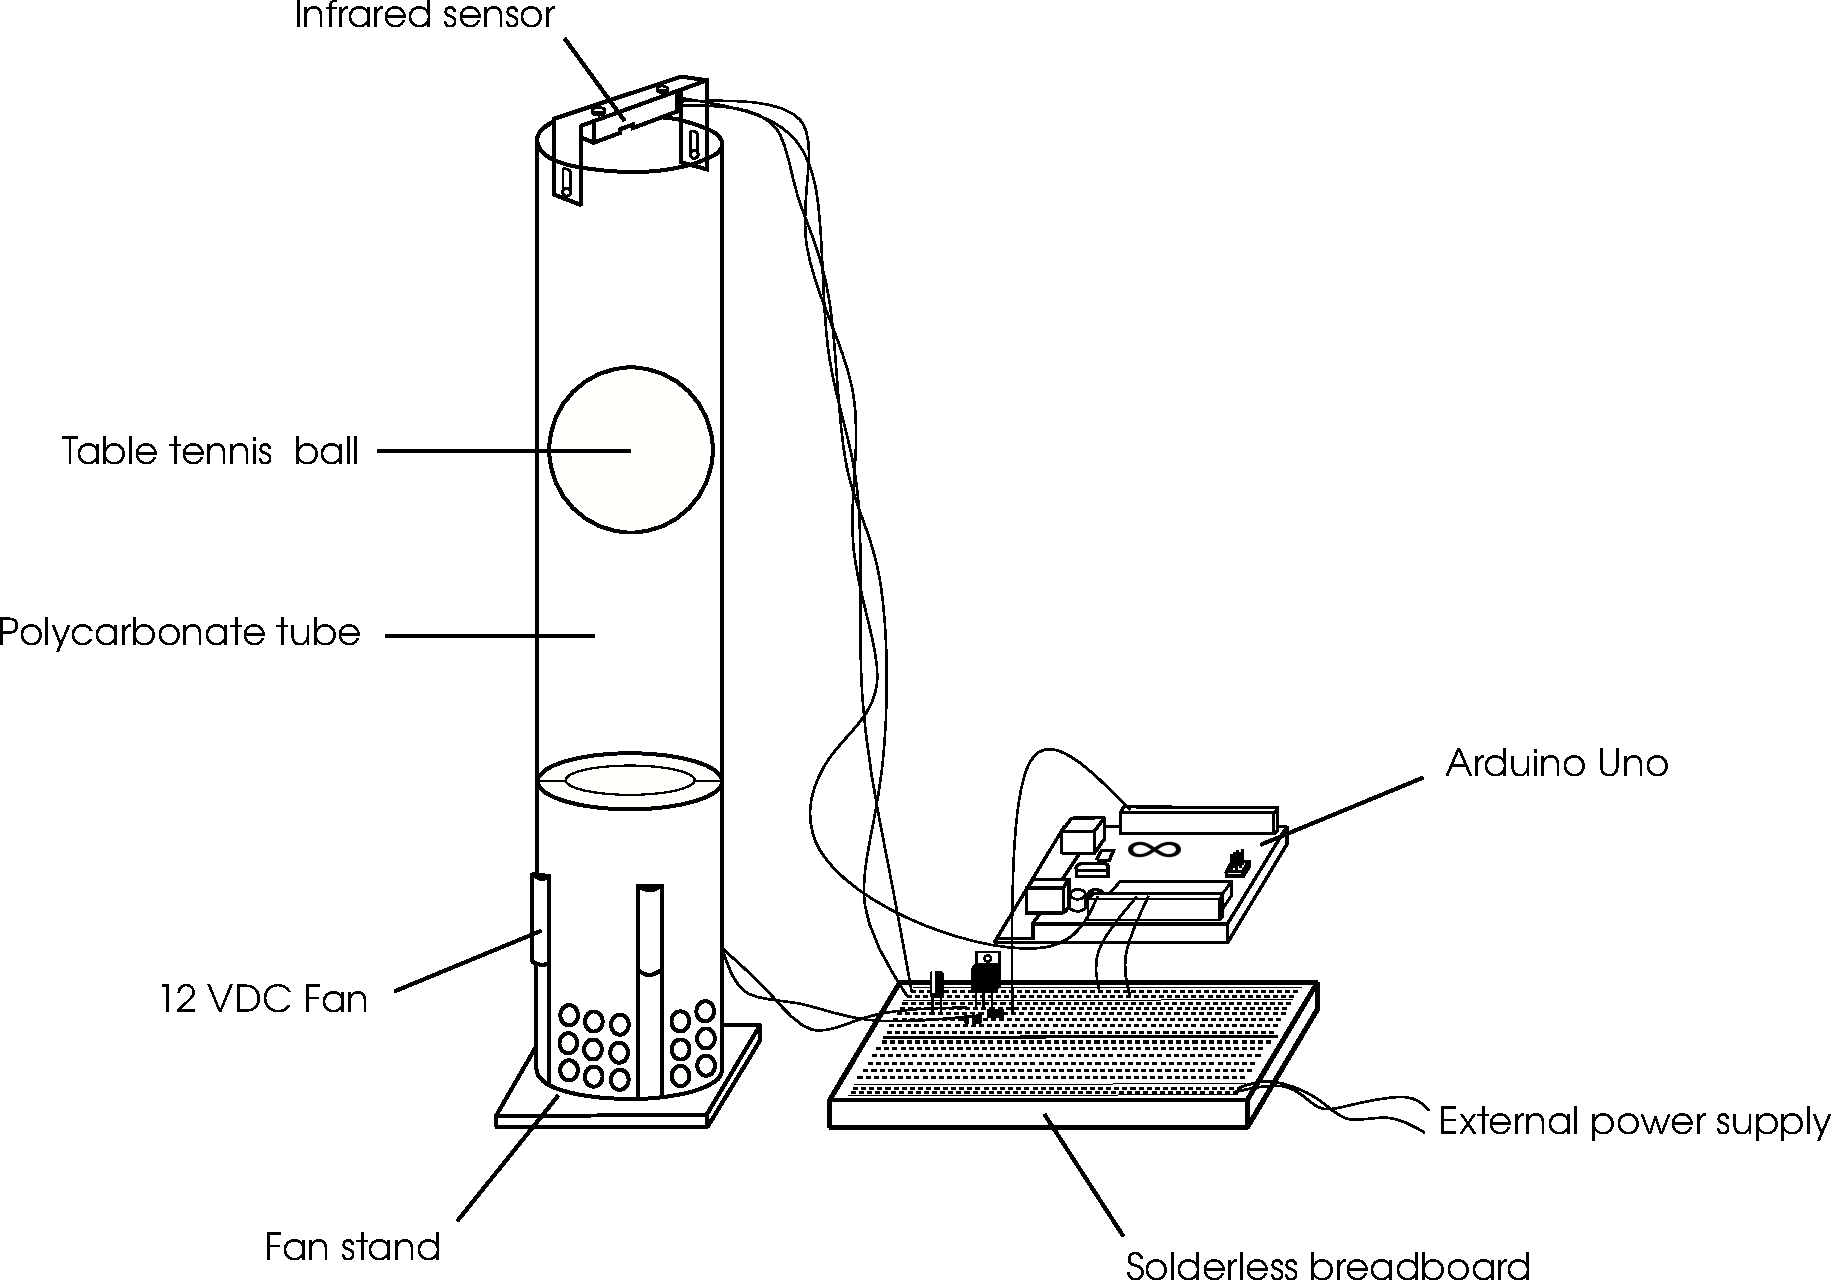
\includegraphics[width=0.9\textwidth]{setup_annot.pdf}
\caption{Schematic of the practical setup.}
\end{figure}

\subsection{Electronic circuit}
The electronic circuit diagram depicted in Fig.~\ref{fig:circuit} is built on a solderless breadboard (Figs.~\ref{fig:breadboard},~\ref{fig:fritzing}). A solderless breadboard consists of two halves split by the center divider and are electrically independent. Each half consists of roughly 50 terminal strips (5 hole columns) and two power rails. The power rails are horizontally connected over the full length of the breadboard, while each terminal strip is vertically connected. There is no vertical connection between the power rails and no horizontal connection between the terminal strips.\\

\mijnfiguur[h!]{width=9cm}{breadboard.pdf}{A solderless breadboard. The power rails are horizontally connected, while the terminal strips are vertically connected.}{fig:breadboard}

The electronic circuit diagram depicted in Fig.~\ref{fig:circuit} can be broken down to two seperate parts: 1) A circuit for the IR proximity sensor, and 2) A transistor circuit to control the fan speed. The IR proximity sensor has 3 pins, a ground (GND) pin, a supply voltage ($\text{V}_{\text{CC}}$) pin and an output voltage ($\text{V}_{0}$) pin. We supply the sensor with 5 VDC power drawn from the Arduino Uno. As its output $\text{V}_{0}$, the sensor returns a voltage between 0~VDC and 5~VDC, either unfiltered to the Arduino's analog input pin (A0), or filtered via an RC filter, as illustrated in Fig.~\ref{fig:fritzing}. An RC filter is an analog first-order low-pass filter, attenuating high-frequency noise on the sensor's output voltage. Using a resistor of $R=22~k\Omega$ and a capacitor of $F=2.2~\mu F$ yields an RC filter with a time constant of $\tau = R*C = 0.1~s$,
\begin{equation}
H(s) = \frac{1}{RC s + 1} = \frac{1}{0.1s + 1}.
\end{equation}

The transistor circuit used to drive the fan's motor combines two concepts from the introduction: a transistor controlled using Pulse Width Modulation (PWM) and a flyback diode. To power the motor, we need to send 12~VDC through it and then on to ground. To give the Arduino Uno control of the motor’s power, you use a transistor, which functions as an electrically operated switch activated by means of PWM from your Arduino’s digital pins. The emitter of the transistor is connected to common ground and the collector is connected to the motor. To control the flow between the emitter and collector, a low power PWM signal can supplied at the base pin (Fig.~\ref{fig:transistor}). You connect pin D9, which has PWM capabilities, to the base pin of the transistor and use a 2.2 $k \Omega$ resistor to limit the current. To limit the chances of a creating a reverse current after cutting the motor's power, we place a flyback diode parallel across the motor. The practical implementation of the motor's electronic circuit on the solderless breadboard is shown in Fig.~\ref{fig:fritzing}. Note how the grounds from both power rails on the solderless breadboard and the Arduino Uno are shared, which is essential to making this setup work.

\subsection{Coupling the Arduino to MATLAB}
Make sure the \texttt{Arduino support package for Simulink} is installed locally on the computers that will be used (Simulink $>$ \texttt{APPS} $>$ \texttt{Get Add-Ons} $>$ \texttt{Get Hardware Support Packages} $>$ \texttt{Simulink Support Package for Arduino}). Connect the Arduino to the computer with the USB cable. Select \texttt{MODELLING} > \texttt{Model Settings} > \texttt{Hardware Implementation} > \texttt{Hardware board: Arduino Uno} to reveal the \texttt{HARDWARE} tab. To run a Simulink model on your Arduino board, select \texttt{HARDWARE} > \texttt{Run with IO}. To execute code continuously on your Arduino, set the simulation time to \texttt{inf}.

\begin{landscape}
\mijnfiguur[h!]{scale=1.4}{circuit.pdf}{Electronic circuit diagram. Note how the IR sensor circuit and the transistor circuit are two seperate entities.}{fig:circuit}
\end{landscape}

\begin{landscape}
\mijnfiguur[h!]{scale=0.8}{levitatingPingPongCircuit_bb.pdf}{Electronic circuit built on the solderles breadboard.}{fig:fritzing}
\end{landscape}


\subsection{Calibrating the IR proximity sensor}
The relationship between the IR sensor's output voltage and its distance to the table tennis ball is needed. First, we collected data by hovering the ball at several heights (using a PID controller) and recording the sensor's output voltage (Fig.~\ref{fig:sensor_calibration}). We then expiremented with several mathematical relationships and found the following \textit{logit} relationship adequately described the ball's height in function of the recorded voltage,
\begin{equation}\label{eq:calibration_sensor}
H(V) = H_{\text{max}} + \dfrac{1}{\beta} \left[ \ln \left( \dfrac{V_{\text{max}} - V_{\text{min}}}{V_{\text{max}} - V} - 1 \right) - \ln(\alpha) \right]
\end{equation}
with $H_{\text{max}} = 0.65~m$, $\alpha = 2.19$, $\beta = 8.91$, $V_{\text{min}} = 0.70~V$, $V_{\text{max}} = 4.51~V$. At the bottom of the tube, a change in the ball's height results only in a very small change in the sensor's recorded voltage. Due to the noise on the recorded voltage, measuring height differences in the bottom 20~cm of the tube is difficult. As the ball gets close to the IR proximity sensor, above 58~cm, the sensor's output voltage drops back to 2~V.

\mijnfiguur[h!]{width=\linewidth}{calibration_sensor.pdf}{Relationship between the height of the table tennis ball and the IR sensor's output voltage.}{fig:sensor_calibration}

\subsection{Mathematical model}

\subsubsection{Model structure}\label{section:model_structure}
The fan at the bottom of the tube blows air upwards around the table tennis ball, which hampers the flow of air thereby creating an upwards \textit{drag force} proportional to the square of the relative velocity of the ball (Fig~\ref{fig:ballInTube}). Air molecules hitting the bottom of the ball are slowed down and subsequently deflected around the ball, resulting in the formation of a high pressure region. The incoming laminar airflow will adhere to the surface of the ball\footnote{This is called the \textit{coanda effect} which you may have know as the deflection of a vertical stream of water across the back of a spoon.} up until the \textit{separation point} where the formation of turbulent eddies begins. In the wake of the ball, a turbulent region of low pressure forms and it is the pressure difference between the bottom and top of the ball that generates the drag force. Opposed is the force of gravity, which pulls the ball down with a constant force irregardless of the ball's velocity. The total force exerted on the tennis ball along the $z$ axis is therefore equal to,
\begin{equation}\label{eq:pingPongForce}
F = \frac{1}{2} \rho A C_D v_{\text{rel}}^2 - mg,
\end{equation}
where $\rho_{\text{air}}$ is the density of air, equal to 1.225 $kg \cdot m^{\text{-}3}$. A is the surface area of the table tennis ball, equal to $4\pi r^2$ with a radius $r=0.02~m$. $C_D$ is the coefficient of drag, which is 0.47 (-) for Reynolds numbers below $Re<10^5$ (S.~Hoerner, 1965. Fluid-Dynamic Drag). $m$ is the mass of the ping ball and is equal to $0.00283~kg$. g is earth's gravitational constant equal to 9.81 $m \cdot s^{\text{-}2}$. $v_{\text{rel}}$ is the relative velocity of air around the table tennis ball in $m \cdot s^{\text{-}1}$, which depends on the velocity of the airflow inside the tube ($v_{\text{air}}$), as well as on the velocity of the table tennis ball itself ($v_{\text{ball}}$). However, because the velocity of the airflow in the tube is not known exactly we make two assumptions. First, we assume it is related to the PWM signal used to control the fan's speed by means of a power law function. Second, we assume there is no pressure drop along the length of the tube, and hence, the air's speed is independent of the position in the tube (Excercise~3.1). Mathematically,
\begin{equation}\label{eq:assumption_no_pressure_drop}
v_{\text{rel}} = v_{\text{air}} - v_{\text{ball}} = \alpha u(t)^\beta - v_{\text{ball}},
\end{equation}
where $\alpha~(m \cdot s^{\text{-}1})$ and $\beta~(-)$ are parameters of the power law function and $u(t)$ is the value of the PWM signal, located between 0 and 255, and corresponding to a 0 \% and a 100 \% duty respectively. Hence, we can rewrite Eq.~\ref{eq:pingPongForce} as follows,
\begin{equation}\label{eq:pingPongForceExtended}
F = \frac{1}{2} \rho A C_D \left( \alpha u(t)^\beta- v_{\text{ball}} \right)^2 - mg.
\end{equation}
Using Newton's second law of motion, we arrive at the following non-linear second order ODE describing the ball's movement inside the tube,
\begin{equation}\label{eq:ODEmodel}
m \frac{\text{d}^2 z}{\text{d}t^2} = \frac{1}{2} \rho A C_D \left(\alpha u(t)^\beta - \frac{\text{d}z}{\text{d}t}\right)^2 - m g.
\end{equation}
Next, as is common practice in control theory, we rewrite the mathematical model in a state-space representation. The system's states, denoted $\bm{x}$, are the position $z$ and velocity $v$ of the ball. Its only observed output $y$ is the position of the ball $z$, its only input is $u(t)$. By substituting $v = dz /dt$ in Eq.~\ref{eq:ODEmodel}, we arrive at the following non-linear model in state-space representation,
\begin{equation}\label{eq:pingPongModelStates}
\begin{cases}
\bm{\dot{x}}(t) &= \bm{f}\big(\bm{x(t)},~u(t)\big) = \begin{bmatrix} \dot{z}(t) \\ \dot{v}(t) \end{bmatrix} = \begin{bmatrix} v(t) \\ \dfrac{\rho A C_D}{2 m} (\alpha u(t)^\beta - v(t))^2 - g \end{bmatrix},\\
y(t) &= g\big(\bm{x(t)},~u(t)\big) = z(t).
\end{cases}
\end{equation}

\mijnfiguur[t!]{width=0.65\textwidth}{force_diagram.pdf}{(left) Velocity contours of the flow around a smooth sphere placed in a laminar fluid flow. (right) Forces acting upon the sphere.}{fig:ballInTube}

\subsubsection{Equilibrium and operating points}

\paragraph{Equillibrium points} A system is in equillibrium when the derivatives of all states are zero when no input is provided, mathematically, $\bm{\dot{x}}(t) = \bm{f}(\bm{x(t)},~ 0) = 0$. Substitution in Eq.~\ref{eq:pingPongModelStates} yields the following conditions,
\begin{equation}
\begin{cases}
v^* = 0~m \cdot s^{\text{-}1}, \\
g = 0~m \cdot s^{\text{-}2},
\end{cases}
\end{equation}
and there is no condition on the ball's position $z$. Thus, the ball can only be at rest at any point in the tube with the fan switched off in the abscence of gravity. Therefore, on earth, where $g = 9.81~m \cdot s^{\text{-}2}$, the system does not have an equillibrium point. In practice, when the fan is switched off, the ball will be in equillibrium at the bottom of the tube, where its weight is supported by the fan stand.

\paragraph{Operating points} A system is in an operating point when the derivatives of all states are zero when input is provided, mathematically, $\bm{\dot{x}}(t) = \bm{f}\left(\bm{x(t)},~\bar{u}\right) = 0$. Substitution of this condition in Eq.~\ref{eq:pingPongModelStates} yields,
\begin{equation}\label{eq:operating_point}
\begin{cases}
v^* = 0~m \cdot s^{\text{-}1}, \\
\bar{u} = \left(\dfrac{2 m g}{\rho A C_D \alpha^2}\right)^{\dfrac{1}{2 \beta}}.
\end{cases}
\end{equation}
From which we conclude: 1) Any position inside the tube can be an operating point as there is no condition on the ball's position $z$, 2) the ball hovers in an operating point because $v^*=0~m \cdot s$, and 3) the fan speed needed to hover the ball $\bar{u}$ only depends on system parameters. Therefore, there exists one unique fan velocity given by Eq.~\ref{eq:operating_point} that will make the ball hover at a fixed height in the tube, irregardless of the ball's position in the tube. When designing a controller, the aim is to stabilise a desired operating point $(z^*,~0,~\bar{u})$.

\subsubsection{Stability of the operating points}\label{section:stability}
To examine the stability of the operating points of a non-linear system analytically, we first linearize the system and evaluate it at generic point $(\bm{x^*}, u^*) = (z^*, v^*, u^*)$. A linear state-space system has the following form,
\begin{equation}
\begin{cases}
\bm{\dot{x}}(t) &= \bm{A} \bm{x}(t) + \bm{B} u(t), \\
y(t) &= \bm{C} \bm{x}(t) + D u(t),
\end{cases}
\end{equation}
Linearising a non-linear system is done by means of a first-order Taylor approximation in the operating point,
\begin{equation}
\bm{A} = \left. \dfrac{\partial \bm{f}}{\partial \bm{x^T}}\right|_{(z^*, v^*, u^*)} ~ \bm{B} = \left. \dfrac{\partial \bm{f}}{\partial u}\right|_{(z^*, v^*,u^*)} ~ \bm{C} = \left. \dfrac{\partial g}{\partial \bm{x^T}}\right|_{(z^*, v^*, u^*)} ~ \bm{D} = \left. \dfrac{\partial g}{\partial u}\right|_{(z^*, v^*, u^*)}.
\end{equation}
Applied to Eq.~\ref{eq:pingPongModelStates},
\begin{equation}\label{eq:linearised_system}
\begin{cases}
\bm{\dot{x}}(t) &=
\underbrace{
\begin{bmatrix}
0 & 1 \\
0 & \dfrac{\rho A C_D}{m} \left( v^* - \alpha \left( u^* \right)^\beta \right)
\end{bmatrix}}_{\bm{A}}
\begin{bmatrix}
z(t) \\
v(t)
\end{bmatrix}
+
\underbrace{
\begin{bmatrix}
0 \\
\dfrac{\alpha \beta \rho A C_D}{m} (u^*)^{\beta-1} \left(\alpha (u^*)^\beta - v^* \right)
\end{bmatrix}}_{\bm{B}}
u(t), \\
y(t) &=
\underbrace{
\begin{bmatrix}
1 & 0
\end{bmatrix}}_{\bm{C}}
\begin{bmatrix}
z(t) \\
v(t)
\end{bmatrix}
+
\underbrace{0}_{D} u(t), \\
\end{cases}
\end{equation}
where $\bm{A}$ is the \textit{system matrix}, $\bm{B}$ is the \textit{input matrix}, $\bm{C}$ is the \textit{output matrix} and $D$ is the \textit{feedthrough matrix}. The eigenvalues of the matrix $\bm{A}$ at the operating point $(z^*,~0,~ \bar{u})$ determine its stability and are found by solving its characteristic equation,
\begin{equation}
\text{det}\left( \lambda I - A \right) = 
\begin{vmatrix}
\lambda & -1 \\
0 & \lambda + \dfrac{\rho A C_D}{m}  \alpha \bar{u}^\beta
\end{vmatrix}
= 0
\end{equation}
\begin{equation}\label{eq:linearised_system_poles}
\iff \lambda_1 = 0\ \lor\ \lambda_2 = - \dfrac{\rho A C_D}{m} \alpha \bar{u}^\beta.
\end{equation}
If all real parts of the eigenvalues are negative than the system is \textit{asymptotically stable} and if at least one real part is positive and the others negative, the system is \textit{unstable}. For $\alpha>0$, our system has one negative eigenvalue and one zero eigenvalue, and therefore exerts \textit{marginal or neutral stability}, which is between an asymptotically stable and an unstable system. When displaced by the fan, the ball will not return to a common steady state, nor will it go away without limit. To examine the system's stability,we can alternatively write down the linearised system's transfer function and examine its poles in the operating points,
\begin{equation}
H(s) = \bm{C} (s \bm{I} - \bm{A})^{\text{-}1} \bm{B} + \bm{D},
\end{equation}
applied to Eq.~\ref{eq:linearised_system},
\begin{equation}
H(s) = \dfrac{\nicefrac{\alpha \beta \rho A C_D}{m}}{s \left(s - \nicefrac{\rho A C_D}{m} \left(v^* - \alpha (u^*)^\beta\right) \right)},
\end{equation}
whose poles in the operating point $(z^*,~ 0,~ \bar{u})$ are identical to those found by solving the characteristic equation (Eq.~\ref{eq:linearised_system_poles}). In Fig.~\ref{fig:streamPlots}, the phase trajectories of the system are given for three fan velocities, below ($u^* = 131$), at ($\bar{u} = 151$), and above ($u^* = 171$) the unique fan speed needed to hover the ball (Eq.~\ref{eq:operating_point})\footnote{For the calibrated values $\alpha = 0.19$ and $\beta = 0.63$, see Excercise~3.5.}. If a point ($z$, $v$) in the phase trajectory is chosen as the initial condition of the system, then the streamlines indicate the change in position and velocity of the table tennis ball over time. With an insufficient fan speed to hover the ball, any initial combination of position and velocity results in the ball landing at the bottom of the tube. Opposed, at a fan speed above the hovering speed, the ball always ends up at the top of the tube. Starting from any initial velocity, a fan speed of $u = 151$ guarantees the ball will eventually come to a standstill.

\mijnfiguur[h!]{width=\textwidth}{streamPlots.pdf}{Phase trajectories for three different values of the fan speed $u(t)$.}{fig:streamPlots}

\subsubsection{Controllability and observability}\label{section:controllability}

\paragraph{Controllability} The controllability matrix of the linearised system in an operating point $(z^*, 0, \bar{u})$ is computed as follows,
\begin{equation}\label{eq:controllability}
\bm{P}
=
\begin{bmatrix}
\bm{B} & \bm{AB}
\end{bmatrix}
=
\bar{u}^{\left(2\beta-1\right)} \dfrac{\alpha^2 \beta \rho A C_D}{m}
\begin{bmatrix}
0 & 1 \\
1 & - \dfrac{\alpha \rho A C_D}{m} \bar{u}^\beta \\
\end{bmatrix},
\end{equation}
and its rank is equal to the number of states (2). Therefore, the system is controllable, meaning an appropriate choice of fan speeds $u(t)$ can be used drive the ball from any initial state to any desired state within a finite timeframe.

\paragraph{Observability} The observability matrix of the linearised system is computed as follows,
\begin{equation}\label{eq:observability}
\bm{S}
=
\begin{bmatrix}
\bm{C} \\
\bm{CA}
\end{bmatrix}
= 
\begin{bmatrix}
1 & 0 \\
0 & 1
\end{bmatrix},
\end{equation}
and its rank is equal to the number of states (2). The system is therefore observable meaning the IR proximity sensor's measurement of the ball's position can be used in conjunction with a Luenberger state estimator to estimate the velocity of the ball. Hence, the system's known states can be used to estimate it's unknown states.

\section{Hands-on practical}

\subsection*{Overview of the practical}
This hands-on practical consists of four parts. In the first part you will study the physical system by analysing its \textbf{open-loop response} or how it reacts without a feedback controller. This will allow you to assess how the system reacts to inputs by the fan, assess the stability of operating points (Section~\ref{section:stability}). Further, you will learn how to filter the IR proximity sensor's signals. Finally, you will perform several response experiments, which you will then use to \textbf{calibrate the mathematical model of the setup} (Eq.~\ref{eq:pingPongModelStates}). In the second part of the practical, you will use the calibrated mathematical model to perform an in-silico tuning of a PID controller. In addition, you will tune a PID controller by means of the Cohen-Coon and Ziegler-Nichols \textbf{empirical tuning methods}. In the third part of this practicum, you will test the tuned PID controllers on the real system. You will study the \textbf{closed-loop response} of the system by studying the controller's P, I and D contributions more closely. You will further study the implications of dead time on the fan's response and measurement noise on the performance of the controller. The fourth and final part of the practical will introduce you to the design of the more advanced \textbf{Linear Quadractic Regulator} with \textbf{Luenberger estimator}. Its performance as compared to the PID controller will be assessed.

\subsection*{Part I: Open-loop control, time- and frequency response}

\subsection{Open-loop control of the fan's speed}
Before implementing any form of feedback control, we investigate how to control the system manually (open-loop control). We'll use the Simulink model shown in Fig.~\ref{fig:sendPWM} to control the fan speed. The model contains a \texttt{Knob} whose output is connected to a \texttt{Constant} block. The knob's output is limited to the interval 0-255 and represents the fan's motor speed $u_{\text{PWM}}$. Setting $u_{\text{PWM}}$ to 0 results in $0/255 \cdot 12\ \text{V} = 0$ V applied to the fan motor, while setting $u_{\text{PWM}}$ to 255 results in $255/255 \cdot 12\ \text{V} = 12$ V applied to the fan motor. A \texttt{display} block is used to more accurately show the value selected on the knob.\\

\pagebreak

\begin{opgave}[Open-loop control of the fan's speed]{}

\begin{enumerate}

	\item Implement the model in Simulink (Fig.~\ref{fig:sendPWM}) or open \textbf{writePWM.slx}. 
	
	\item Start by turning the knob to $u_{\text{PWM}} \approx 180$. Run the Simulink model by pressing the \texttt{Run with IO} button in the \texttt{Hardware} tab. Pay attention to the system's response. What is the minimum value $u_{\text{PWM}}$ needed to raise the ping pong ball from the stand?

		\leegvakf{1cm}

	\item What is the approximate $u_{\text{PWM}}$ needed to hover the table tennis ball at 30 cm?

		\leegvakf{1cm}

	\item What is the approximate $u_{\text{PWM}}$ needed to hover the table tennis ball at 50 cm? Are your findings in line with those obtained by analytically assessing the stability of the operating points (Section~\ref{section:stability})?

		\leegvakf{1cm}
	
\end{enumerate}

\end{opgave}

\mijnfiguur[h!]{scale=0.6}{sendPWM.pdf}{Simulink model used to control the fan speed.}{fig:sendPWM}

\subsection{Measuring and filtering the IR sensor's signal}
Next, we will measure the step response of the system. For this purpose, you can use the Simulink model \textbf{readProximity.slx} (Fig.~\ref{fig:readProximity}). An \texttt{analog read} block is used to read the sensor's output voltage at pin A0. However, the voltage was already transformed into a 10 bit digital signal by the Arduinos on-board analog-to-digital converter so a number between 0 and 1023 is returned. 
After changing the signal's datatype to \texttt{double}, we convert it back to a voltage between 0~V and 5~V. Next, the signal is smoothed by combining a \texttt{median filter} and a first-order system (low-pass filter). Next, Eq.~\ref{eq:calibration_sensor} is used to convert the voltage into a distance from the IR sensor (Fig~\ref{fig:sensor_calibration}). However, because of a singularity in Eq.~\ref{} at 0.70~V, the voltage is limited to a minimum of 0.701~V.  Finally, distance from the sensor is converted to height in the tube and a \texttt{saturation} block is used limit the height to a physcially plausible range.\\

\begin{opgave}[Measurement of the ping pong ball's height]{}

\begin{enumerate}
	\item Implement the model in Simulink (Fig.~\ref{fig:readProximity}) or open \textbf{readProximity.slx}.
	\item Manually control the height of the ping pong ball while observing the height using the \texttt{Scope}. How is the overall signal quality? Does  the signal quality differ at different heights? What could you do to improve this signal?
	
	\leegvakf{1cm}

\end{enumerate}
\end{opgave}

\begin{opgave}[Filtering the IR sensor's signal]{}

\begin{enumerate}
	\item Add a first-order transfer function after the block converting the voltage to the range 0-5~VDC. Set the gain to $K=1$ and time constant to $\tau = 0.2~s$. Optionally connect the time constant to a \texttt{knob} for convenience. Visualise the filtered and unfiltered signal using a \texttt{scope}. Manually control the height of the ping pong ball while observing the height using the scope. How is the signal quality now?
	
	\leegvakf{1cm}
	
	\item Vary the first-order transfer function's time constant. How does the signal quality change? How does the timing of the filtered signal differ from the unfiltered signal? Find an appropriate time constant to use for the rest of the practical.
	
	\leegvakf{2cm}
	
	\item What is the name of such a filter? Can you explain how this filter works?
	
	\leegvakf{2cm}
	
\end{enumerate}

\end{opgave}

\mijnfiguur[h!]{width=\linewidth}{readProximity.pdf}{Simulink model used to read the ball's height in open-loop control.}{fig:readProximity}

\subsection{Collecting time response data}

Having a mathematical model of the system is usefull to design a well-functioning controller. We previously derived a set of non-linear second-order ordinary differential equations representing the physical processes underlying the table tennis ball movement (Eq.~\ref{eq:pingPongModelStates}). This model, based on a combination of physical laws and unknown parameters is a \textbf{grey box model}. In practice, systems are often too complex to come up with a grey or white box model. Many complex, non-linear system's dynamics are reasonably approximated by linear models under typical operating conditions. However, our system, with its neutral stability, is not well approximated by a first- or second order transfer function and hence, no such model is identified during this practical. \\

You will perform experiments and use them to calibrate the unknown parameters $\alpha$ and $\beta$ in Eq.~\ref{eq:pingPongModelStates}. The first experiment is a \textbf{block-shaped response} experiment, which combines a step response experiment with a U-shaped response experiment (Fig.~\ref{fig:experiments}a). This experiment is preferred over the more simple step response experiment because it contains information on both the upward and downard trajectory of the table tennis ball, which differ from each other. Additionally, the U-shaped response contains information on the ball's \textbf{in-flight dead time} in response to changes in the fan speed. In the second \textbf{W-shaped response} experiment, a similar step-wise input is given, followed by a series of three step-wise changes in the fan speed, alternating below and above the fan speed needed to hover the ball $\bar{u}$(Eq.~\ref{eq:operating_point}) (Fig.~\ref{fig:experiments}b). The block-shaped response experiments will be used as \textbf{calibration dataset}, while the W-shaped response experiment will be used as a \textbf{validation dataset} to assess the predictive accuracy of our calibrated model. \\

\newpage
\begin{opgave}[Sytem response experiments]{}

	\begin{enumerate}
		\item Open the script \textbf{writeBlockResponse.m}, which is preprogramed to perform a step response, followed by a U-shaped response (Fig.~\ref{fig:experiments}a). The intial step response is performed by stepping the fan speed to $u_{\text{max}}$ for 7.5~s, followed by 7.5~s at the equillibrium fan speed $\bar{u}$ to stabilise the ball's spin for the second part of the experiment. Then, the U-shaped response is performed by stepping down the fan's speed to $u = \bar{u} - u_{\text{step}}$ for 2.5~s, then stabilising the ball at the equillibrium fan speed $\bar{u}$ for 5.0~s, followed by a 2.5~s step up to $u = \bar{u} + u_{\text{step}}$. By default, three initial step motor speeds $u_{\text{max}} = 170,~185,~255$, and two U-sizes $u_{\text{step}} = 6, 10$ are permutated, and every combination is performed in duplicate to average out natural variations in the response. Thus, a total of 12 experiments are performed. You will provide the observed time needed before the ball was lifted from the stand (\textit{lift-off dead time}), which is then automatically cut from the experiment. In the script, provide an accurate estimate of the fan's equillibrium speed \texttt{u\_eq} (Excercise~1), and set the \texttt{output\_name} to \textit{blockResponse.csv}. The script uses the Simulink model \textit{blockResponse.slx}. Limit the ball's height to 50~cm using a thin wooden stick.
		
		\item Open the script \textbf{writeWResponse.m}, which uses the Simulink model \textit{wResponse.slx} to log a W-shaped response experiment which we will use as a validation dataset (Fig.~\ref{fig:experiments}b). Five identical experiments are automatically performed to visualise the natural variation on the reponse. After all five experiments, you will provide one lift-off dead time which is then cut from the experiments. Use the automatically generated figure containing the fan speed and height response to \textbf{determine the in-flight dead time}.
		
			\fbox{%
  				\parbox{0.92\textwidth}{
   				$t_d$ =
  				}%
			}

	\end{enumerate}
	
\end{opgave}

\mijnfiguur[h!]{width=0.85\linewidth}{experiments.pdf}{(a) Fan speed and ball height during a block-shaped response experiment. (b) Fan speed and ball height during a W-response experiment.}{fig:experiments}

\subsection{Understanding the system's open-loop frequency response}
Finally, you will investigate the system's open-loop frequency response. You will do this by applying a sinusoidal input of varying frequency to the fan and observing the amplitude of the resulting sinusoidal changes in the ball's height, as well as the phase shift between the input and output signals. Using your observations, you construct an approximate \textbf{Bode diagram} allowing you to make further deductions on the system's dynamics. 

\begin{opgave}[Frequency response of the system]{}
	\begin{enumerate}
		\item  Open the Simulink model \textbf{frequency.slx} and use the \texttt{knob} to set the equillibrium fan speed needed to hover the ball, $\bar{u}_{\text{PWM}}$ (Excercise~3.1). Set the frequency knob to 10~rad/s, which results in the fan speed sinusoidally varying between $\bar{u}_{\text{PWM}} \pm 30$, within $t = \pi/10 = 0.3~s$ (= high-frequency input). Temporarily increase the value of $\bar{u}_{\text{PWM}}$ to overcome the additional energy needed to get the ball airborne. Next, hover the ball where the IR sensor's signal's quality is good, around 30~cm. Note that as the transistor heats up, its ability to pass a current increases. Hence, starting from a cold setup, you may need to initially use a value slightly higher than $\bar{u}_{\text{PWM}}$. What is the amplitude of the sinusoidal changes in the ball's height?
		
		\leegvakf{1cm}
		
		\item Decrease the frequency of the input signal to 1~rad/s in a step-wise manner. Prevent the ball from going fully down or up by making adjustments to $\bar{u}_{\text{PWM}}$. How does the amplitude of the ball's height change? Are the input and output signals in or out of phase?
		
		\leegvakf{1cm}
		
		\item Decrease the frequency of the input signal below 1~rad/s. Stop making temporary adjustments to $\bar{u}_{\text{PWM}}$ to prevent the ball from reaching either end of the tube. What is the amplitude of the ball's height? Not accounting for the dead time introduced by the initial energy needed to get the ball hovering, are the input and output signals in or out of phase?
		
		\leegvakf{1cm}
		
		\item Draw an approximate Bode diagram of the system. What kind of system is the Bode diagram characteristic of?
	\end{enumerate}
\end{opgave}

		\begin{figure}[t!]
			\centering
			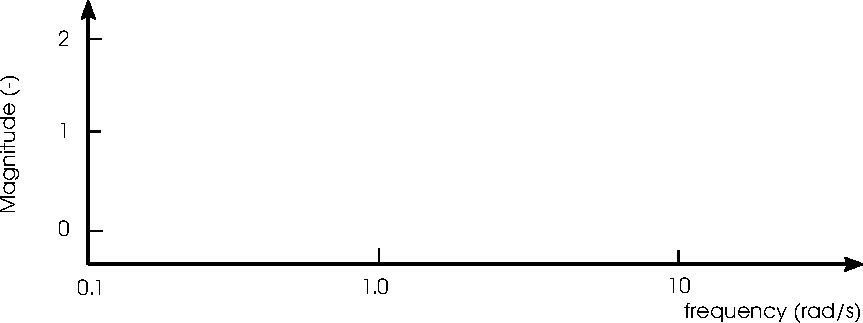
\includegraphics[width=0.75\linewidth]{bode_diagram_empty_1.pdf}
			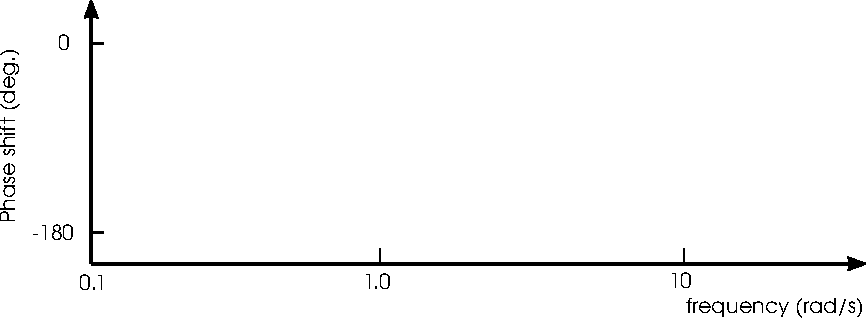
\includegraphics[width=0.75\linewidth]{bode_diagram_empty_2.pdf}
			\caption{Approximate Bode diagram based on the setup's open-loop frequency response.}
 		\end{figure}

\subsection*{Part II: System identification and PID controller tuning}

The second part of this practical can be done \textbf{independently from the lab set-up}. In this part of the practical, the unkown parameters in the mathematical model of the setup (Eq.~\ref{eq:pingPongModelStates}) are identified using the response data gathered in Excercise~3.4. Then, the calibrated mathematical model is implemented in Simulink and used to design a suitable PID controller \textbf{in-silico}. Finally, two \textbf{emperical tuning techniques}, by Cohen-Coon and Ziegler-Nichols, are used to tune a PID controller. 

\subsection{System Identification}

\begin{opgave}[Calibrating the mathematical model (Eq.~\ref{eq:pingPongModelStates})]{}

	\begin{enumerate}

		\item Use \textbf{systemIdentification.m} to calibrate the unkown parameters $\alpha$ and $\beta$ in Eq.~\ref{eq:pingPongModelStates} using the block-shaped response dataset gathered in Excercise~3.4.1. In the script, be sure to provide your estimate of the in-flight dead time (Excercise~3.4.2) and validate the paths to \textit{blockResponse.csv} and \textit{wResponse.csv}. The script will automatically minimize the sum-of-squared errors between the block-shaped response experiments and the mathematical model by finding optimal values for $\alpha$ and $\beta$. After the estimation of $\alpha$ and $\beta$ is completed, a figure comparing the experiments and the mathematical model is provided (Fig.~\ref{fig:calibration}). Write down the optimal values of $\alpha$ and $\beta$ below.
		
			\fbox{%
  				\parbox{0.92\textwidth}{
  				\vspace{0.2cm}
   				$\alpha$ =\\
   				$\beta$ =
   				\vspace{0.2cm}
  				}%
			}

		\item Calculate the equillibrium fan speed $\bar{u}$ using Eq.~\ref{eq:operating_point}. Use the following values for the constants: $\rho = 1.225~kg \cdot m^{\text{-}3}$, $m = 0.00283~kg$, $A = 4 \pi r^2$ with $r = 0.02~m$, $g = 9.81~m \cdot s^{\text{-}2}$, and $C_D = 0.47~(\text{-})$. Is the computed value sufficiently close to the observed value (Excercise~3.1.3)?

			\fbox{%
  				\parbox{0.92\textwidth}{
  				\vspace{0.2cm}
   				$\bar{u} = \left(\dfrac{2 m g}{\rho A C_D \alpha^2}\right)^{\dfrac{1}{2 \beta}} = $
   				\vspace{0.2cm}
  				}%
			}
	
	\item How is the goodness-of-fit of the mathematical model to the experimentally obtained data? What is the purpose of the validation experiment?
	
		\leegvakf{2cm}
		
\end{enumerate}
\end{opgave}

\mijnfiguur[h!]{width=\linewidth}{calibration.pdf}{Goodness-of-fit of the mathematical model (Eq.~\ref{eq:pingPongModelStates}) to the calibration and validation experiments (Fig.~\ref{fig:experiments}). The mean average error of the mathematical model in predicting the validation dataset is 2.2~cm.}{fig:calibration}

\pagebreak
\subsection{Tuning a PID controller}

In this section, you will learn how to tune a PID controller with the following transfer function,
\begin{equation}
C(s) = K_P + K_I~ \dfrac{1}{s} + K_D \underbrace{\left( \dfrac{s}{\left(1/K_F\right) s + 1} \right)}_{\text{filtered derivative}},
\end{equation}
where $K_P$ is the proportional gain, $K_I$ is the integral gain, $K_D$ is the derivative gain, and $1/K_F$ is the derivative filter first-order time constant. The PID controller can be implemented either directly in Simulink using the \texttt{PID} block, or using the following basic Simulink blocks,

\mijnfiguur[h!]{width=0.7\linewidth}{PID_simulink.pdf}{Implementation of a PID controller in Simulink. The derivation of the filtered derivative's transfer function is given in red.}{fig:PID_simulink}

\begin{opgave}[In-silico PID tuning]{}

	\begin{enumerate}
		\item Implement the mathematical model of the setup (Eq.~\ref{eq:pingPongModelStates}) with a PID controller in Simulink (Fig.~\ref{fig:PID_simulink}). Saturate the ball's height between 0~cm and 60~cm. Do this by implementing the equivalent of the following Matlab code in Simulink using two consecutive \texttt{Switch} blocks,
	\begin{lstlisting}[style=matlab]
	if z >= upper_bound
		zdot = min(0, v); % pass only negative velocities at upper bound
	elseif z <= lower_bound
		zdot = max(0, v); % pass only positive velocities at lower bound
	else
		zdot = v;
	end
	\end{lstlisting}
	
		Placing a \texttt{Saturation} block after the integration of Equations~\ref{eq:pingPongModelStates} in Simulink is incorrect and not equivalent to the above Matlab code. Do not model the in-flight dead time or noise on the sensor's output initially. Make sure the initial value of the integral control action is set to zero. Simulate a stepwise increase in the setpoint from 0~cm to 40~cm, and use the following controller gains $K_P=100$, $K_I=10$, $K_D=0$, $K_F=100$. Observe the output of the integral control action. What value does the integral control action converge to?
		
		\leegvakf{1cm}
		
		\item Simulate a step-wise increase in the setpoint height from 20~cm to 40~cm. Set the initial output of the integral control action to the equillibrium fan speed $\bar{u}$. Tune the PID controller, what values for $K_P$, $K_I$, $K_D$ and $K_F$ yield satisfactory behavior?
		
			\fbox{%
  				\parbox{0.92\textwidth}{
  				\vspace{0.2cm}
   				$K_P = $\\
   				$K_I = $\\
   				$K_D = $\\
   				$K_F = $
   				\vspace{0.2cm}
  				}%
			}
		
		\item Use a \texttt{Transport delay} block to model the in-flight dead time as a delay on the motor's output (be sure to set its initial output to the equillibrium fan speed $\bar{u}$). What is the impact of the dead-time on the stability of your previously tuned PID controller?
		
		\leegvakf{1cm}
		
		\item Use a \texttt{Spectral noise} (recommended) or \texttt{Random number} block to make the height measurement noisy. Subsequently filter the noisy signal using a low-pass filter (Excercise~3.3). Now, retune the PID controller. What values for $K_P$, $K_I$, $K_D$ and $K_F$ yield satisfactory behavior? 
		
			\fbox{%
  				\parbox{0.92\textwidth}{
  				\vspace{0.2cm}
   				$K_P = $\\
   				$K_I = $\\
   				$K_D = $
   				\vspace{0.2cm}
  				}%
			}		
		
		\item What is the impact of a noisy measurement on the derivative control action? What happens for high values of the proportional gain $K_P$ in the abscense of integral and derivative control action, and in the abscense of a setpoint change?
		
		\leegvakf{2cm}
		
		\item Simulate a stepwise decrease in the fan's effectiveness after a step response experiment, thereby increasing the fan's equillibrium speed $\bar{u}$. Model this by increasing the fan's proportionality constant $\alpha$ (Eq.~\ref{eq:pingPongModelStates}) by 5-10~\% using a \texttt{Step} block. Reassess the performance of your tuned controller.
		
		\leegvakf{2cm}
		
		\item (Optional) The Simulink model \textbf{ODEModelPID\_smithpredictor.slx} contains an implementation of the mathematical model of the setup (Eq.~\ref{eq:pingPongModelStates}), with a PID controller and with a Smith predictor to compensate for the dead time on the fan's motor response. Asses the stability of your previously tuned PID controller when a Smith predictor is used.
		
		\leegvakf{1cm}
		
	\end{enumerate}

\end{opgave}

\paragraph{Cohen-Coon tuning} The empirical tuning method by Cohen and Coon is an \textbf{open-loop tuning technique} relying on many complex non-linear system's step response being adequately approximated by a sigmoidal first-order transfer function with dead time (at least under/near the relevant operating conditions).
\begin{equation}
H(s) = \dfrac{y(s)}{u(s)} = \dfrac{K e^{-t_d s}}{\tau s + 1},
\end{equation}
where $K$ is the system's gain, $\tau$ its time constant, and $t_d$ its dead time. After applying a stepwise increase to the fan speed $u_{\text{step}}$ PWM units above the equillibrium fan speed $\bar{u}$, the gain $K$ can be computed as $K = \Delta y_{\text{step}}/u_{\text{step}}$, while the time constant $\tau$ and dead time $t_d$ can be estimated graphically. The former is the time needed to reach 63.2~\% of the step's output change $\Delta y_{\text{step}}$, while the latter is the elapsed time before a change in input has an effect on the system's output (Fig.~\ref{fig:cohen_coon_tuning}).\\

For our setup, it is best to use the in-flight dead time gathered in Excercise~3.4.2 instead of the lift-off dead time, as the latter is not representative of the system's behavior once the ball is airborne. Our choice to subtract the fan's equillibrium speed $\bar{u}$ from the step size is based on the intuition that this will better mimic a first-order response (remember the ball does not go anywhere for fan speeds under $\bar{u}$). Cohen and Coon devised that a stable closed-loop response can be obtained by computing the $K_P$, $K_I$ and $K_D$ values using the tuning rules listed in Table \ref{tab:cohen_coon}.

\mijnfiguur[h!]{width=\linewidth}{cohen_coon_tuning.pdf}{Using the block response experiments to estimate the gain, time constant and dead time of the approximate first-order response.}{fig:cohen_coon_tuning}

\begin{opgave}[Cohen-Coon tuning]{}
\end{opgave}
	\begin{enumerate}
		\item Use the block response experiments gathered during Excercise~3.4.1 to graphically estimate the gain $K$ and time constant $\tau$, both for the initial step (labeled 1 in Fig.~\ref{fig:cohen_coon_tuning}), as well as the upwards step during the U-shaped phase of the experiment (labeled 2 in Fig.~\ref{fig:cohen_coon_tuning}). Tune the PID controller using the tuning rules of Cohen-Coon listed in Table~\ref{tab:cohen_coon}.
		
		\leegvakf{2cm}
		
		\item Simulate the step response of the closed-loop system using the tuned P, PI and PID controllers. What controllers lead to a stable closed-loop response?
		
		\leegvakf{2cm} 
		
	\end{enumerate}


\begin{table}[h!]
\caption{Tuning rules of Cohen-Coon for a PID controller $C(s) = K_P + K_I/s + K_D s$.}
\centering
 \begin{tabular}{|c | c c c|} 
 \hline
  & $K_P$ & $K_I$ & $K_D$ \\  
 \hline
 P & $\dfrac{1}{K} \dfrac{\tau}{t_d} \left( 1 + \dfrac{t_d}{3 \tau} \right) $ & - & - \\ [3mm] 
 PI & $\dfrac{1}{K} \dfrac{\tau}{t_d} \left( 0.9 + \dfrac{t_d}{12 \tau} \right) $ & $K_P*\left(\dfrac{1}{t_d}~\dfrac{9 + 20 (t_d/\tau)}{30 + 3 (t_d/\tau)} \right)$ & - \\ [3mm] 
 PID & $\dfrac{1}{K} \dfrac{\tau}{t_d} \left( 4/3 + \dfrac{t_d}{4 \tau} \right) $ & $K_P*\left(\dfrac{1}{t_d}~\dfrac{13 + 8 (t_d/\tau)}{32 + 6 (t_d/\tau)} \right)$ & $K_P*\left( t_d~\dfrac{4}{11 + 2 (t_d/\tau)}\right)$ \\ [3mm] 
 \hline
 \end{tabular}
 \label{tab:cohen_coon}
\end{table}

\paragraph{Ziegler-Nichols tuning} Opposed to the method of Cohen and Coon, the empirical tuning method of Ziegler and Nichols is a \textbf{closed-loop tuning technique}. First, the system is stabilised in a desired operating point. Then, the controller is reduced to its P-action, and a change in the setpoint is demanded. The proporational controller gain $K_P$ is then increased until the system's closed loop response to the demanded setpoint change results in permanent oscillations. This gain, often referred to as the \textit{ultimate gain} $K_u$, as well as the period of the continuous oscillations $P_u$ are recorded and used to tune the system (Table~\ref{tab:ziegler_nichols_tuned}).

\begin{opgave}[Empirical PID tuning methods: Ziegler-Nichols]{}
	\begin{enumerate}
		\item Determine the ultimate control gain $K_u$ and the period of the associated oscillations $P_u$ using your simulink model of the setup (Excercise~3.7). Tune the controller using the tuning rules in Table~\ref{tab:ziegler_nichols}.
		
		\leegvakf{3cm}
		
		\item Simulate a step-wise change in the setpoint from 20~cm to 40~cm, do the controllers yield a satisfactory response?
		
		\leegvakf{2cm}
		
	\end{enumerate}
\end{opgave}

\begin{table}[h!]
\caption{Tuning rules of Ziegler-Nichols for a PID controller $C(s) = K_P + K_I/s + K_D s$.}
\centering
 \begin{tabular}{|c | c c c|} 
 \hline
  & $K_P$ & $K_I$ & $K_D$ \\
 \hline
 P & $\dfrac{K_u}{2}$ & - & - \\ [3mm] 
 PI & $\dfrac{K_u}{2.2}$ & $\dfrac{1.2 K_P}{P_u}$ & - \\ [3mm] 
 PID & $\dfrac{K_u}{1.7}$ & $\dfrac{2 K_P}{P_u} $ & $\dfrac{8 K_P}{P_u} $ \\ [3mm] 
 \hline
 \end{tabular}
 \label{tab:ziegler_nichols}
\end{table}

\subsection*{Part III: PID control of the experimental set-up}

In this part of the practical, you will test your tuned PID controllers on the experimental setup and assess their performance. You will examine the frequency response of the closed-loop system and construct its Bode diagram, which you will then compare to the open-loop Bode diagram (Excercise~3.5). By using PID controllers in practice you will gain a deeper understanding of some common issues such as noisy measurements and dead time. 

\subsection{Testing PID control on the experimental setup}

\begin{opgave}[PID control of the experimental set-up]{}
	\begin{enumerate}
		\item  Open the Simulink model \textbf{PID.slx}, which contains the implementation of a PID-controller. Set adequate parameters for the low pass filtering of the IR sensor's measurement (Excercise~3.3). Verify the initial condition of the integral controller's \texttt{Integrate} block is set to the fan's equillibrium speed $\bar{u}$ (Excercise~3.6.2). The height setpoint, controller gains ($K_P$, $K_I$, $K_D$, $K_F$) and the time constant of the height measurement's low pass filter $\tau_F$ can be tuned using the knobs while operating the experimental setup. Use the knobs to configure your optimal PID-controller. Change the setpoint from 0~cm to 40~cm and observe the response. Disturb the system by constricting the airflow with your hands. Does your controller work adequately?

		\leegvakf{2cm}
		
	\end{enumerate}	
\end{opgave}

\begin{opgave}[Contribution of the different control actions]{}
	\begin{enumerate}
		\item Set the initial condition of the integral controller's \texttt{Integrate} block to zero for the duration of this excercise. Use the \textit{Scope} to visualise the \textbf{individual contributions of the proportional, integral and derivative actions} of the controller. Start with the ball at the bottom of the tube. Set the proporational gain to $K_P = 600-800$, while disabling the integral and derivative control ($K_I=K_D=0$). Raise the setpoint to 40~cm. Does the ball ever reach the setpoint? How is this phenomenon called?

			\leegvakf{1cm}

		\item Start with the ball at the bottom of the tube. Disable the proportional and derivative control by setting $K_P = K_D = 0$. Set the integral gain to $K_I = 50$. Raise the setpoint to 40~cm. What happens to the contribution of the I-action? Is the obtained system stable?
		
			\leegvakf{1cm}

		\item Starting with the ball stabilised at 40~cm, disable the integral and derivative control action by setting $K_I = K_D = 0$. Make stepwise changes in the setpoint and disturb the system. Is the system stable and its response satisfactory? Do you feel like any derivative action is needed at this point? 

			\leegvakf{1cm}
			
		\item Starting with the ball stabilised at 40~cm, disable the integral and derivative control action by setting $K_I = K_D = 0$. Make the fan slightly less effective by holding your hand flat above the tube at some distance (circa 5~cm). Is the controller able to keep the ball at 40~cm? Restabilise the system at 40~cm and make the fan slightly less effective, but set the integral gain to $K_I=10$. What happens to the output of the integral controller? Reduce the fan's efficacy at least 30~s and then remove your hand. What phenomenon do you observe?
		
		\leegvakf{1cm}
			
	\end{enumerate}
\end{opgave}

\begin{opgave}[Effect of filtering on the derivative action]{}
	\begin{enumerate}
		\item Start with the ball stabilised at 40~cm, set the derivative filter's gain to $K_F = 1$ and increase the derivative gain to $K_D = 200\text{-}300$. Take some stepwise changes in the setpoint. What do you observe?
		
			\leegvakf{2cm}
			
		\item Examine the effect of changing the derivative filter's gain $K_F$, the time constant of the first order derivative filter is equal to $\tau = 1/K_F$.
		
			\leegvakf{2cm}
	\end{enumerate}
\end{opgave}

\begin{opgave}[Effect of dead time on stability]{}
	\begin{enumerate}
		\item In \textbf{PID.slx}, add a \texttt{Transport delay} block of 1~s to the measurement of the ball's height to introduce additional dead time. Use stable controller gains and raise the setpoint from 0~cm to 40~cm. What is the effect of the added dead time on the stability of the controlled system?
	
		\leegvakf{1 cm}
	
	\end{enumerate}
\end{opgave}

\subsection{Understanding the system's closed-loop frequency response}

Finally, in analogy to Excercise~3.5, you will investigate the system's closed-loop frequency response. You will do this by applying a sinusoidal change of the height setpoint and observing the amplitude of the resulting sinusoidal changes in the ball's height, as well as the phase shift between the input and output signals. Using your observations, you will construct an approximate \textbf{Bode diagram}. 

\begin{opgave}[Frequency response of the system]{}
	\begin{enumerate}
		\item  Open the Simulink model \textbf{frequencyPID.slx} and use the knobs to set your optimal controller gains. Make sure the initial condition of the integral controller's \texttt{Integrate} block is set to the fan's equillibrium speed $\bar{u}$. The setpoint varies sinusoidally around 35~cm with an amplitude of 10~cm and a variable frequency. The frequency can be changed using the knob, start a high frequency of 10~rad/s. What is the amplitude of the sinusoidal changes in the ball's height? Are the input and output signals in or out of phase?
		
		\leegvakf{1cm}
		
		\item Decrease the frequency of the input signal to 3~rad/s. How does the amplitude of the ball's height change? Are the input and output signals in or out of phase?
		
		\leegvakf{1cm}
		
		\item Decrease the frequency of the input signal to around 2~rad/s. What is the amplitude of the ball's height? Are the input and output signals in or out of phase?
		
		\leegvakf{1cm}
		
		\item Decrease the frequency of the input signal to around 1~rad/s. What is the amplitude of the ball's height? Are the input and output signals in or out of phase?
		
		\leegvakf{1cm}
		
		\item Decrease the frequency of the input signal to around 0.5~rad/s. What is the amplitude of the ball's height? Are the input and output signals in or out of phase?
		
		\leegvakf{1cm}
		
		\item Draw an approximate Bode diagram of the system. What kind of system is the Bode diagram characteristic of?
	\end{enumerate}
\end{opgave}

		\begin{figure}[h!]
			\centering
			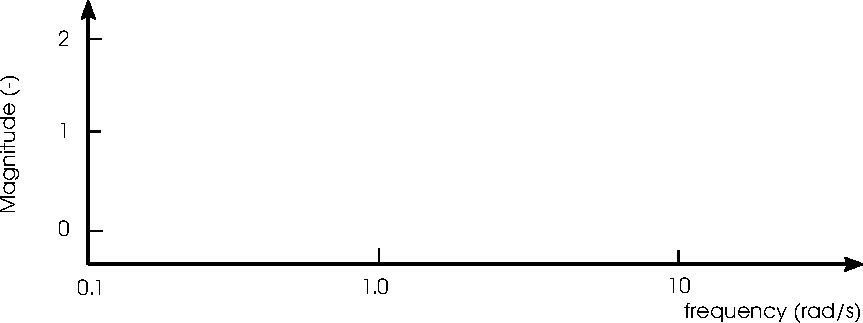
\includegraphics[width=0.75\linewidth]{bode_diagram_empty_1.pdf}
			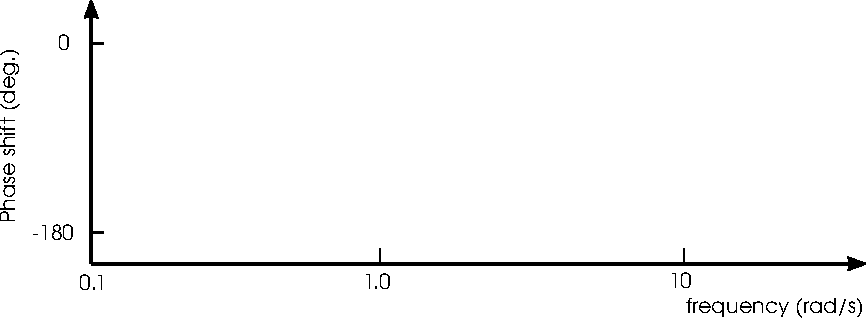
\includegraphics[width=0.75\linewidth]{bode_diagram_empty_2.pdf}
			\caption{Approximate Bode diagram based on the setup's closed-loop frequency response.}
 		\end{figure}

\subsection*{Part IV: Advanced control strategies}

\subsection{Linear-Quadratic Regulator with Luenberger state observer}

\subsubsection{Control strategy and design}
\paragraph{Linear-Quadratic Regulator} In this section, we design an optimal state feedback controller to control the height of our table tennis ball. Mathematically, we attempt to drive our non-linear system to a desired operating point $\bm{x_{\text{sp}}} = (z, v)$ using an input $u(t)$. To accomplish this, the input $u(t)$ is chosen as the sum of two components (Fig.~\ref{fig:nonLinearControl_withTTS}): The first, $\bar{u}$, is the input needed to keep the system in an operating point, and is the solution to the equation $\bm{\dot{x}(t)} = \bm{f}(\bm{x(t)}, \bar{u}) = 0$ (Eq.~\ref{eq:operating_point}). The second, $u^*$, is the force needed to drive the system from any initial condition to the desired operating point, mathematically, $u^* = \bm{K} (\bm{x} - \bm{x_{\text{sp}}})$, which is the product of the feedback gain matrix $\bm{K}$ and the deviation from the setpoint.\\

The values of the feedback matrix K must then be chosen so that the real parts of the eigenvalues of the (linearised) system with state feedback $(\bm{A} + \bm{B} \cdot \bm{K})$ are negative, stabilizing the operating point. This is possible if the system is controllable, which we have previously verified (Eq.~\ref{eq:controllability}). For nonlinear systems the feedback matrix $\bm{K}$ is typically designed using the system matrix $\bm{A}$ and input matrix $\bm{B}$ from the system linearised in the operating point (Eq.~\ref{eq:linearised_system}). However, this strategy should always be used with care as nonlinear systems may have multiple operating points\footnote{Linear systems have only one operating point!}and the size of the stable region around the desired operating point is unknown. Our system has an infinite number of operating points, as the ball can be stabilised at any height $z$ inside the tube as long as the fan's hover speed $\bar{u}$ is maintained. However, because each operating point is neutrally stable, designing the gain matrices based on a linearised system is likely to work.\\

Instead of intuitively choosing the entries of the gain matrix $\bm{K}$ to obtain negative eigenvalues for the system with state feedback, it is possible to design an \textit{optimal} gain matrix $\bm{K}$. Doing so entails defining the desired qualities of an \textit{optimal} controller and translating them into an objective function. Typically, these qualities are: 1) Reaching the setpoint quickly, where a state-cost matrix $\bm{Q}$ governs the relative importance of reaching the setpoint of different states. For our setup, asigning more importance to reaching the height setpoint than the velocity setpoint ($v=0~m \cdot s^{\text{-}1}$) will result in oscillations. 2) Minimise the cost needed to reach the setpoint, where an input-cost matrix $\bm{R}$ governs the relative importance (read price) of using different inputs to reach the setpoint. Because our system has only one input, the input-cost matrix is not relevant to this practical. 3) To avoid offset. Minimising this objective function yields an optimal gain matrix $\bm{K}$, which is referred to as the Linear-Quadratic Regulator.\\

\begin{opgave}[Designing an appropriate state feedback gain matrix $\bm{K}$]{}
	\begin{enumerate}
		\item What size should the state feedback gain matrix $\bm{K}$ be?
		
		\leegvakf{1cm}
		
		\item Use the system matrix $\bm{A}$ and input matrix $\bm{B}$ of the linearised system (Eq.~\ref{eq:linearised_system}) to design a suitable state feedback gain matrix $\bm{K}$. Do this symbolically in Wolfram Mathematica by evaluating Eq.~\ref{eq:linearised_system} in an operating point $\bm{x^*} = \left(z^*,~ 0,~ \bar{u}\right)$, and then computing conditions for the entries of $\bm{K}$ to make the eigenvalues of $\bm{A} + \bm{B K}$ negative.
		
		\leegvakf{2cm}
		 
		 \item Implement the mathematical model of the setup (Eq.~\ref{eq:pingPongModelStates}; Excercise 3.7.1) with state feedback (Fig.~\ref{fig:nonLinearControl_withTTS}) in Simulink. Implement dead time on the fan's motor response (Excercise~3.4.2). Assume the position and velocity of the ball are both known so no Luenberger state observer is needed. Simulate a step in the setpoint from 20~cm to 40~cm. Assess the response for different state feedback gain matrices. Use the builtin Matlab function \texttt{lqr(A, B, Q, R)} to design state feedback gain matrices. Experiment with varying the state-costs of the height setpoint $Q_{11}$ and the velocity setpoint $Q_{22}$ when designing LQR gains. Find a suitable gain matrix to try out on the experimental setup.
		 
		 \leegvakf{1cm}
		 
	\end{enumerate}
\end{opgave}
		
\paragraph{Luenberger state observer} Only the position of the table tennis ball is monitered by the IR sensor while state feedback requires all system states, both the position and velocity of the table tennis ball, to be known. To resolve this problem, a Luenberger state observer can be designed because the system is observable (Eq.~\ref{eq:observability}). Similar to the state feedback, the observer is designed using the linearised system. The state observer is a linear system consisting of a predictor and a corrector,
\begin{equation}
\underbrace{\bm{\dot{\hat{x}}} = \bm{A\hat{x}} + \bm{B u}}_{\text{predictor}} + \underbrace{ \bm{L} \left(\bm{y} - \bm{C \hat{x}} - \bm{D u} \right)}_{\text{corrector}} 
\end{equation}
which models the evolution of the system's states $\bm{\hat{x}} = (\hat{z},~ \hat{v})$ by using the sensor's measurement of the ball's height $y$, the fan speed $u$, and a (linearised) process model as its inputs. The predictor, $\bm{\dot{\hat{x}}} = \bm{A \hat{x}} + \bm{B u}$, uses the system's (linearised) process model, inputs $u(t)$ and an initial condition to compute the dynamic trajectory of the system's states. However, the predicted state trajectory will diverge from the actual state trajectory as time progresses. Therefore a corrector term, $\bm{ L \left(y - C \hat{x} - D u} \right)$, equal to $\bm{L}$ times the difference between the sensor's measurement $y$ and the predicted measurement using the model $\hat{y} = C \hat{x} - D u$, is added to the equation. Designing the matrix $\bm{L}$ so that the eigenvalues of the matrix $(\bm{A} - \bm{L C})$ are strongly negative drives the predictive error of the observer $\bm{\epsilon} = \bm{x -\hat{x}}$ to zero. For a controllable and observable system, the \textbf{separation principle} states that matrices $\bm{K}$ and $\bm{L}$ can be designed independently.


\begin{figure}[h]
	\centering
	\begin{tikzpicture}[auto, node distance=2.5cm,>=latex']
	
	\node [block] (system) {
		$\begin{aligned}
		\dot{\bm{x}}&=\bm{f}(\bm{x},\bm{u})\\
		\bm{y}&=\bm{x}
		\end{aligned}$
		};
		
	\node [block, below = 1.0cm of system] (ttk) {
	$K(\bm{\hat{x}} - \bm{x_{sp}})$
	};
	
	\node [block, right = 1.0cm of system] (tts) {
	$\dot{\bm{\hat{x}}} = \bm{A \hat{x}} + \bm{B u} + \bm{L} (\bm{y} - \bm{C \hat{x}} - \bm{D u})$
	};
	
	\node [output, right = 1.5 cm of tts] (output) {};
	
	\node [above = 0.5cm of tts] (u) {$\bm{u}$};
	\draw [->] (u) -- node [] {}(tts);
	
	\draw [->] (tts) -- node [name=tts_output] {$\bm{\hat{x}}$}(output);
	
	\draw [->] (system) -- node [name=system_tts] {$\bm{y}$}(tts);
	
	\node [circle, draw, black, minimum size=5mm, inner sep=0pt,below = 0.5 cm of tts_output] (sum1) {$-$};
	
	\node [right = 0.5cm of sum1] (xbar) {$\bm{x}_{sp}$};
	
	\draw [->] (xbar) -- node [] {}(sum1);
	\draw [->] (tts_output) -- node [] {}(sum1);
	\draw [->] (sum1) |- node [] {}(ttk);
	
	\node [circle, draw, black, minimum size=5mm, inner sep=0pt,left = 1 cm of system] (sum2) {$+$};
	
	\draw [->] (ttk) -| node [near end] {$\bm{u}^\ast$}(sum2);
	\draw [->] (sum2) -- node [] {$\bm{u}$}(system);
	
	\node [block, left = 1.0 cm of sum2] (solve) {
	$\begin{aligned}
	& \text{Solve} \\
		& \bm{\dot{x}(t)} = \bm{f}(\bm{x(t)}, \bar{u}) = 0
		\end{aligned}$};
	%\draw [->,preaction={draw,white,line width=5pt}] (xbar) |- node {} (solve);
	\draw [->] (solve) -- node [near end] {$\bar{\bm{u}}$} (sum2);
	\end{tikzpicture}
	\caption{Schematic representation of a state feedback strategy with Luenberger state observer to bring a non-linear system to a setpoint $\bm{x_{\text{sp}}}$.}
	\label{fig:nonLinearControl_withTTS}
\end{figure}


\begin{opgave}[Designing an appropriate corrector gain matrix $\bm{L}$]{}
	\begin{enumerate}
		\item What size should the corrector gain matrix $\bm{L}$ be?
		
		\leegvakf{1cm}
		
		\item Use the system matrix $\bm{A}$ and output matrix $\bm{C}$ of the linearised system (Eq.~\ref{eq:linearised_system}) to design a suitable state observer corrector gain matrix $\bm{L}$. Do this symbolically in Wolfram Mathematica by evaluating Eq.~\ref{eq:linearised_system} in an operating point $\bm{x^*} = \left(z^*,~ 0,~ \bar{u}\right)$, and then computing conditions for the entries of $\bm{L}$ to make the eigenvalues of $\bm{A} - \bm{L C}$ negative.
		
		\leegvakf{3cm}
		
		\item Adjust your Simulink implementation of the mathematical model of the setup with state feedback (Excercise~3.15.4) to include a Luenberger state observer. Based on the separation principle, the state feedback gain matrix $\bm{K}$ and the corector gain matrix $\bm{L}$ can be designed independently. Assume only the position of the ball is measured and add artifical measurement noise, which you subsequently filter (Excercise~3.7.4). Simulate a step in the setpoint from 20~cm to 40~cm and visualise the difference between the measured and estimated heights of the table tennis ball, as well as the estimated velocity, for different corrector gain matrices $\bm{L}$.
		
		 \leegvakf{1cm}
		
	\end{enumerate}
\end{opgave}

%\begin{figure}[h]
%	\centering
%	\begin{tikzpicture}[auto, node distance=2.5cm,>=latex']
%	
%	\node [block] (system) {
%		$\begin{aligned}
%		\dot{\bm{x}}&=\bm{f}(\bm{x},\bm{u})\\
%		\bm{y}&=\bm{x}
%		\end{aligned}$
%		};
%		
%	\node [block, below = 1.0cm of system] (ttk) {
%	$K(\bm{x} - \bm{x_{sp}})$
%	};
%	
%	\node [output, right = 3.5 cm of system] (output) {};
%	
%	\draw [->] (system) -- node [name=y] {$\bm{x}$}(output);
%	
%	\node [circle, draw, black, minimum size=5mm, inner sep=0pt,below = 0.5 cm of y] (sum1) {$-$};
%	
%	\node [right = 0.5cm of sum1] (xbar) {$\bm{x}_{sp}$};
%	
%	\draw [->] (xbar) -- node [] {}(sum1);
%	\draw [->] (y) -- node [] {}(sum1);
%	\draw [->] (sum1) |- node [] {}(ttk);
%	
%	\node [circle, draw, black, minimum size=5mm, inner sep=0pt,left = 1 cm of system] (sum2) {$+$};
%	
%	\draw [->] (ttk) -| node [near end] {$\bm{u}^\ast$}(sum2);
%	\draw [->] (sum2) -- node [] {$\bm{u}$}(system);
%	
%	\node [block, left = 1.0 cm of sum2] (solve) {
%	$\begin{aligned}
%	& \text{Solve} \\
%		& \bm{\dot{x}(t)} = \bm{f}(\bm{x(t)}, \bar{u}) = 0
%		\end{aligned}$};
%	%\draw [->,preaction={draw,white,line width=5pt}] (xbar) |- node {} (solve);
%	\draw [->] (solve) -- node [near end] {$\bar{\bm{u}}$} (sum2);
%	\end{tikzpicture}
%	\caption{Schematic representation of a state feedback strategy to bring a non-linear system to a setpoint $\bm{x_{\text{sp}}}$.}
%	\label{fig:nonLinearControl}
%\end{figure}

\subsubsection{Testing LQR control on the experimental setup}

\begin{opgave}[LQR control of the experimental setup]{}
	\begin{enumerate}
		\item Open the Simulink model \textbf{LQR.slx}, which contains the implementation of an LQR controller. Be sure to change the solution algorithm to the fixed-step Backward Euler \texttt{ode1be} method. The state feedback gain matrix's elements $k_{11}$ and $k_{12}$ can be tuned using the knobs. Raise the setpoint from 0~cm to 40~cm and observe the system's response. How does the response compare to that of a PID controller?
		
		\leegvakf{1cm}
		
	\end{enumerate}
\end{opgave}

%\begin{opgave}[Frequency response of the LQR controller]{}
%	\begin{enumerate}
%		\item Open the Simulink model \textbf{frequencyLQR.slx}, which uses an LQR controller to vary the height setpoint sinusoidally around 35~cm with an amplitude of 10~cm and a variable frequency. Similar to Excercise~3.14 the frequency can be changed using the knob, start at a high frequency of 10~rad/s, and lower the setpoint frequency stepwise to 0.5~rad/s. Record the relative amplitude and phase shift of the sinusoidal changes in the ball's height and use them to draw an approximate Bode diagram below. Is the response more or less stable than with a PID controller? How can you deduce this from the Bode diagram?
%		
%		\leegvakf{1cm}
%		
%	\end{enumerate}
%\end{opgave}
%	
%\begin{figure}[h!]
%	\centering
%	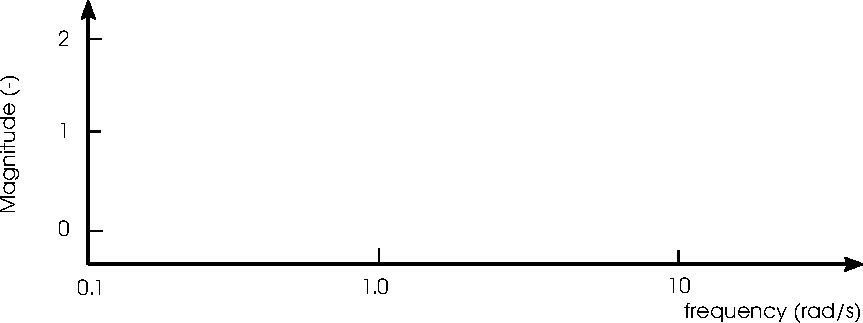
\includegraphics[width=0.72\linewidth]{bode_diagram_empty_1.pdf}
%	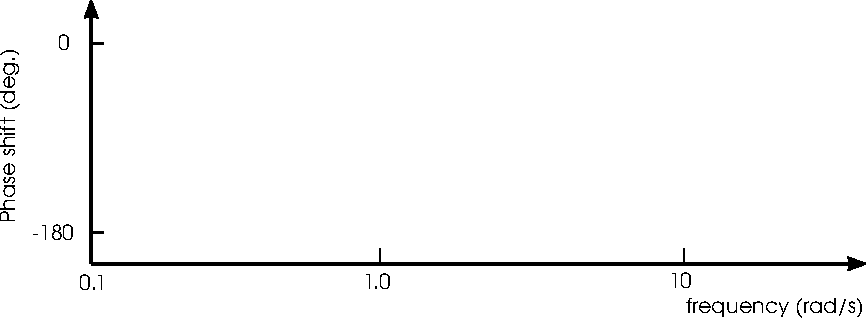
\includegraphics[width=0.72\linewidth]{bode_diagram_empty_2.pdf}
%	\caption{Approximate Bode diagram based on the setup's closed-loop frequency response with an LQR controller.}
% 		\end{figure}

\section{Solutions}

\subsection*{Linearisation, controllability and observability in Wolfram Mathematica}

The following Wolfram Mathematica code was used to compute the derivatives of Eq.~\ref{eq:pingPongModelStates} symbolically, in order to obtain a linearised mathematical model of the setup (Eq.\ref{eq:linearised_system}, Section~\ref{section:stability}). Mathematica was further used to check the controllability and observability of the setup (Section~\ref{section:controllability}). 

\begin{lstlisting}[style=mathematica]
(*Linearise system symbolically*)
Clear[v, u, rho, r, A, Cd, m, g, alpha, beta]
f = {{v}, {(0.5*rho*A*Cd/m)*(alpha*u^beta - v)^2 - g}} ;
FullSimplify[D[f, z]]
FullSimplify[D[f, v]]
FullSimplify[D[f, u]]

(*Define linearized model in generic point x=(z,v,u)*)
a = {{0, 1}, {0, (rho*A*Cd/m)*(v - alpha*u^beta)}};
b = {{0}, {(alpha*beta*rho*A*Cd/m)*u^(beta - 1)*(alpha*u^beta - v)}};
c = {{1, 0}};
d = {{0}};
model = StateSpaceModel[{a, b, c, d}]

(*Check controllability*)
v = 0;
FullSimplify[ControllabilityMatrix[model]]
MatrixRank[ControllabilityMatrix[model]]
ControllableModelQ[model]

(*Check observability*)
ObservabilityMatrix[model]
MatrixRank[ObservabilityMatrix[model]]
ObservableModelQ[model]
\end{lstlisting}

\subsection*{Excercise 3.1}

\begin{enumerate}
\setlength\itemsep{0em}
	\item NA.
	\item Approximately 162 (may differ from setup to setup).
	\item Approximately 152 (may differ from setup to setup).
	\item Approximately 153 (may differ from setup to setup). Because the fan speed needed to hover the ball at 30~cm and 50~cm are almost identical, the assumption that there is no pressure drop along the length of the tube is valid. In other words, the air's speed in the tube is quasi-independent of the position in the tube and hence Eq.~\ref{eq:assumption_no_pressure_drop} is valid.
\end{enumerate}

\subsection*{Excercise 3.2}

\begin{enumerate}
\setlength\itemsep{0em}
\item NA.
\item The signal is noisy and its overall quality is poor, especially when the table tennis ball is in the bottom 20~cm of the tube. This is caused by the low sensitivity of the sensor in this region (Fig.~\ref{fig:sensor_calibration}). Between 58~cm - 63~cm, the sensor falsly thinks the ball's height drops to around 40~cm.
\end{enumerate}

\subsection*{Excercise 3.3}

\begin{enumerate}
\setlength\itemsep{0em}
\item An example of a Simulink model can be found in Fig.~\ref{fig:readProximity_sol}. The signal quality has improved.
\item The low pass filter introduces a delay in the signal (dead time). A lower time constant results in a noisier signal but less dead time. A higher time constant results in a smoother but more delayed signal. Finding an appropriate time constant is a balancing act between signal quality and dead time. Both a poor quality signal quality and dead time lower a feedback controller's ability to stabilise the system. We recommend a (fast) filter time constant $\tau_F = 0.05\text{-}0.10~s$ when using a PID controller on the experimental setup.
\item A low-pass filter, which amplifies low-frequency signals and attenuates high-frequency signals. In our case, the sensor's noise is in the high-frequency spectrum. 
\end{enumerate}


\subsection*{Excercise 3.4}

\begin{enumerate}
\setlength\itemsep{0em}
	\item See Fig.~\ref{fig:blockResponse}.
	\item $t_d \approx 0.5~s$, see Fig.~\ref{fig:wResponse}.
\end{enumerate}

\subsection*{Excercise 3.5}

\begin{enumerate}
\setlength\itemsep{0em}
\item The amplitude of the sinusoidal changes in the ball's height (output signal) is very small, almost non-existent. The ball hovers in the tube.
\item As the frequency of the input signal is lowered, the amplitude of the output increases. The input and output signals are almost fully out of phase (-180~degrees).
\item The amplitude of the output now covers the entire length of the tube. The ball starts at the bottom of the tube and reaches the top of the tube during each cycle. Ignoring the dead time induced by the additional energy needed to get the ball in the air, the input and output signals are now more or less in phase (0~degrees).
\item The approximate Bode diagram is characteristic of a first-order system (Fig.~\ref{fig:approx_bode_diagram_open}). The system's breakout frequency is located at approximately 1~rad/s. As previously discussed, a first-order system is a low-pass filter, as low-frequency inputs are amplified while high-frequency inputs are attenuated. 
\end{enumerate}

\subsection*{Excercise 3.6}

\begin{enumerate}
\setlength\itemsep{0em}
\item $\alpha=0.19,~\beta=0.63$. May differ between setups.
\item $\bar{u} = 151$, and thus in line with the value found during Excercise~3.1.
\item The mathematical model is able to adequately describe the time course of the validation experiment (Fig.~\ref{fig:calibration}), as gauged by a small mean average error of 2.2~cm. Performing \textit{out-of-sample} testing on a \textit{validation} dataset allows us to confidently assert the validity and predictive performance of our mathematical model. Other performance indicators could be the values of the parameters, which must make sense if the parameters have physical meaning, or the size of confidence intervals on the parameter estimates (obtained using the Fisher Information Matrix or Markov-Chain Monte-Carlo sampling).
\end{enumerate}

\subsection*{Excercise 3.7}

\begin{enumerate}
\setlength\itemsep{0em}
\item The integral control action converges to $\bar{u}$ (Fig.~\ref{fig:tuned_PID1}). The PID controller's integral action thus `learns' what fan speed is needed to hover the ball. Therefore, it is best to initialise the integral control action as $\bar{u}$ (\texttt{Initial condition} in the I-controller's \texttt{Integrate} block). The Simulink model, including the in-flight dead time and noisy measurements, is shown in Figs.~\ref{fig:ODEModelPID}, \ref{fig:ODEModelPID_system}, and \ref{fig:ODEModelPID_zdot}.
\item $K_P=1000;~ K_I=0;~ K_D=100;~K_F=1$ (Fig.~\ref{fig:tuned_PID2}). 
\item More in-flight dead time destabilises the closed-loop response (Fig.~\ref{fig:tuned_PID3}).
\item $K_P=50;~ K_I=0;~K_D=0;~K_F=1$ (Fig.~\ref{fig:tuned_PID4}).
\item The derivative control action destabilises the closed-loop response. Large proportional gains can also destabilise the closed-loop system, even in the abscence of a setpoint change, this is due to the combination of the sensor's noise and the system's dead time (Fig.~\ref{fig:tuned_PID5}).
\item As the I-controller is essentially `learning' how to hover the ball by finding $\bar{u}$, setting $K_I = 0$ makes the system incapable of adjusting $\bar{u}$. However, external disturbances, such as the electronic components ``warming up'', may cause changes of $\bar{u}$ over time. Therefore, the use of only a P-controller will make the system incapable of handling external disturbances (Fig.~\ref{fig:tuned_PID6}). An alternative controller's response ($K_P=80;~ K_I=10;~ K_D=50;~K_F=1$) is shown in Fig.~\ref{fig:tuned_PID7}.
\item The use of a Smith predictor enhances the closed-loop stability of the system. Higher proportional gains $K_P$ can now be applied before the system becomes unstable. 
\end{enumerate}

\subsection*{Excercise 3.8}

\begin{enumerate}
\setlength\itemsep{0em}
\item The controller gains tuned using the empirical method by Cohen and Coon are shown in Tables \ref{tab:cohen_coon_tuned1} and \ref{tab:cohen_coon_tuned2}.
\item The response to a step-wise increase in the setpoint height from 20~cm to 40~cm for the controllers listed in Table~\ref{tab:cohen_coon_tuned1} are shown in Fig.~\ref{fig:tuned_PID_cohencoon} (with dead time but without noisy measurements). Only the P-controller leads to an adequate closed-loop response, the tuned integral gains $K_I$ are too high to achieve a stable closed-loop response. Note how there is no offset when using a P-controller (Q: How is this related to the system's stability?). The Cohen-Coon tuning rules are based on the assumption that the system's response are adequately approximated by a linear first-order system. As our system is non-linear with neutral stability, the approximation likely does not hold. Always use empirical tuning rules based on linear approximations with care when designing a suitable controller.
\end{enumerate}

\begin{table}[h!]
\caption{Controller gains tuned using the empirical method by Cohen and Coon. For an initial step size of $u_{\text{max}} = 170$, $K = 0.5 / (170 - 151) = 0.026$, $\tau = 0.8~s$ and $t_d = 0.5~s$.}
\centering
 \begin{tabular}{|c | c c c|} 
 \hline
  & $K_P$ & $K_I$ & $K_D$ \\ [0.5ex] 
 \hline
 P & 73 & - & - \\ [3mm] 
 PI & 58 & 78 & - \\ [3mm] 
 PID & 91 & 91 & 14 \\ [3mm] 
 \hline
 \end{tabular}
 \label{tab:cohen_coon_tuned1}
\end{table}

\begin{table}[h!]
\caption{Controller gains tuned using the empirical method by Cohen and Coon. For an upwards step during the U-shaped response part of the block response experiments with $u_{\text{step}} = 10$, $K = (0.5 - 0.1) / 10 = 0.0025$, $\tau = 1.5~s$ and $t_d = 0.5~s$.}
\centering
 \begin{tabular}{|c | c c c|} 
 \hline
  & $K_P$ & $K_I$ & $K_D$ \\ [0.5ex] 
 \hline
 P & 67 & - & - \\ [3mm] 
 PI & 56 & 56 & - \\ [3mm] 
 PID & 85 & 92 & 15 \\ [3mm] 
 \hline
 \end{tabular}
 \label{tab:cohen_coon_tuned2}
\end{table}

\subsection*{Excercise 3.9}

\begin{enumerate}
\setlength\itemsep{0em}
\item The ultimate control gain $K_u \approx 114$ and the period of the resulting permanent oscillation $P_u \approx 3.5~s$ were determined in silico using the calibrated mathematical model (Fig.~\ref{fig:tuned_PID_zieglernichols_1}). It is possible to determine the ultimate control gain using the setup. The gains of the controllers tuned using the rules of Ziegler and Nichols are given in Table~\ref{tab:ziegler_nichols_tuned}.

\item The resulting system's closed-loop response using the tuned controller gains is shown in Fig.~\ref{fig:tuned_PID_zieglernichols_2}. The P and PI controllers provide a stable closed-loop response while the PID controller does not. The P controller's response is preferred over the PI controller's response. Similar to the tuning method of Cohen and Coon, the integral gain $K_I$ is too high. Based on the empirical method from Ziegler-Nichols, the use of a P-controller seems most adequate. 
\end{enumerate}

\begin{table}[h!]
\caption{Controller gains tuned using the empirical method by Ziegler and Nichols. For an ultimate control gain $K_u \approx 114$ and period of the resulting permanent oscillation of $P_u \approx 3.5~s$.}
\centering
 \begin{tabular}{|c | c c c|} 
 \hline
  & $K_P$ & $K_I$ & $K_D$ \\ [0.5ex] 
 \hline
 P & 57 & - & - \\ [3mm] 
 PI & 52 & 17.8 & - \\ [3mm] 
 PID & 67 & 38.3 & 153 \\ [3mm] 
 \hline
 \end{tabular}
 \label{tab:ziegler_nichols_tuned}
\end{table}

\subsection*{Excercise 3.10}

\begin{enumerate}
	\setlength\itemsep{0em}
	\item The controller with gains $K_P=80;~ K_I=10;~ K_D=50;~ K_F=1$, and filter time constant $\tau_F=0.05~s$ works adequately for setpoint changes and disturbances (Excercise 3.7.6). Note how the integral controller's output converges to $\bar{u}$ (at least after some time, as the electronic components warm up).
\end{enumerate}

\subsection*{Excercise 3.11}

\begin{enumerate}
	\setlength\itemsep{0em}
	\item No, the ball will repeatedly go up and down the tube. The ball's average position will be located below the setpoint, and this is termed ``offset''.
	\item The I ccontroller's output gradually increases to a value over the fan's equillibrium speed $\bar{u}$, raising the ball of the stand. As the ball crosses the desired setpoint, the I controller's starts gradually decreasing but too slow; the ball makes it way to the top of the tube. As the I controller's output gradually decreases back under the fan's equillibrium speed $\bar{u}$, the ball starts making its way down the tube again and the cycle is repeated. The obtained system is oscillatory and thus unstable, the I controller suffers from ``windup''.
	\item With the proportional gain set to $K_P = 80$, the system's reaction to setpoint changes and disturbances is adequate and stable. Integral or derivative action does not seem needed.
	\item Without the integral controller `learning' the new (increased) equillibrium fan speed $\bar{u}$, the controller is unable to maintain a height of 40~cm. With the integral controller enabled, its output gradually increases and the ball maintains its height of 40~cm. Removing the disturbance suddenly results in ``integral windup''. 
\end{enumerate}

\subsection*{Excercise 3.12}
\begin{enumerate}
	\setlength\itemsep{0em}
	\item The system becomes less stable because the derivative controller amplifies the high-frequent noise from the sensor. Intuitively, this makes sense: measurement noise is a small change in the absolute value of the measurement over a very small period of time. Noise thus has a large rate of change (derivative), resulting in a large D-controller action. What you observe is the D-controller reacting to the noise of the IR sensor. However great a D-controller may seem at stabilising a system, this is only true on paper. Ultimately, the use of derivative action can be beneficial, but it has to be used in the right situations and in the right amounts. Your starting assumption should be to see if the process will run satisfactorily on PI control alone. Adding derivative should be done cautiously and with appropriate filtering of the signal.  
	\item Lowering the derivative filter gain to $K_F = 0.5$ makes the system more stable because the sensor's noise is filtered more (derivative filter time constant is lowered to 2~s). Increasing the derivative filter gain to $K_F = 2$ makes the system less stable.
\end{enumerate}

\subsection*{Excercise 3.13}
\begin{enumerate}
	\setlength\itemsep{0em}
	\item Added dead time destabilises the closed-loop system.
\end{enumerate}

\subsection*{Excercise 3.14}
\begin{enumerate}
	\setlength\itemsep{0em}
	\item The magnitude of the amplitude is close to zero, the signals are out of phase.
	\item The magnitude of the amplitude is close to one, the signals are out of phase.
	\item The magnitude of the amplitude is higher than one, the signals are shifted by roughly 90 degrees.
	\item The magnitude of the ampltiude is close to one, the signals are in phase.
	\item The approximate Bode diagram is characteristic of a second-order system (Fig.~\ref{fig:approx_bode_diagram_closed}).
\end{enumerate}

\subsection*{Excercise 3.15}
\begin{enumerate}
	\setlength\itemsep{0em}
		\item The system's states $\bm{x} = (z, v)$ are of size $2\times1$, and the size of $u^* = \bm{K} \left(\bm{x} - \bm{x_{\text{sp}}} \right)$ must be $1\times1$. Therefore, the feedback gain matrix $\bm{K}$ must be of size $1\times2$.  The feedback gain matrix is typically of size $m \times n$, where $m$ is the number of inputs and $n$ is the number of system states.  
		\item The following Wolfram Mathematica code can be used to compute the values of $k_{11}$ and $k_{12}$ that result in the real parts of the eigenvalues of the matrix $\bm{A} + \bm{B} \cdot \bm{K}$ to be equal to -5 and -2, thereby stabilising the system. We obtain $k_{11} = 118~\text{and}~k_{12} = 30$.
		
\begin{lstlisting}[style=mathematica]
(*Define model parameters*)
rho = 1.225;
r = 0.02;
A = 4*Pi*r^2;
Cd = 0.47;
m = 0.00283;
g = 9.81;
alpha = 0.19; 
beta = 0.63; 

(*Define the steady state fan speed*)
ubar = (2*m*g/(rho*A*Cd*alpha^2))^(0.5/beta);

(*Define operating point*)
u = ubar;
v = 0;

(*Define linearized model in generic point x=(z,v,u)*)
a = {{0, 1}, {0, (rho*A*Cd/m)*(v - alpha*u^beta)}};
b = {{0}, {(alpha*beta*rho*A*Cd/m)*u^(beta - 1)*(alpha*u^beta - v)}};
c = {{1, 0}};
d = {{0}};
model = StateSpaceModel[{a, b, c, d}]

(*Compute conditions on entries in matrix K guaranteeing negative \
eigenvalues of A + B.K *)
Clear[k11, k12]
eigK = FullSimplify[Eigenvalues[a - b . {{k11, k12}}]];
Reduce[Re[eigK[[1]]] == -5 && Re[eigK[[2]]] == -2  , {k11, k12}, Reals]
\end{lstlisting}
		
		If $k_{11} = 115$, we can use Mathematica to find what values of $k_{12}$ are needed to stabilise the system. We find that if $k_{11} = 115$ then $k_{12} > 21$ to stabilise the system.
		
\begin{lstlisting}[style=mathematica]
Reduce[Re[eigK[[1]]] < 0 && Re[eigK[[2]]] < 0 && k11 == 115, {k12}, Reals]	
\end{lstlisting}

		Additionaly, Wolfram Mathematica can find \textit{optimal} values of the feedback gain matrix $\bm{K}$ by optimising an LQR problem. For a state cost matrix $\bm{Q} = [[14000, 0]; [0, 2000]]$, we find optimal gains $k_{11} = 118,~\text{and}~k_{12} = 34$. 
		
\begin{lstlisting}[style=mathematica]
(*Design gains using LQR*)
q = {{14000, 0}, {0, 2000}};
r = {{1}};
K = LQRegulatorGains[model, {q, r}, "FeedbackGains"] 
OLpoles = LQRegulatorGains[model, {q, r}, "OpenLoopPoles"]
CLpoles = LQRegulatorGains[model, {q, r}, "ClosedLoopPoles"]
\end{lstlisting}

\item The step response from 0~cm to 40~cm, in the presence of 0.5~s of delay on the fan's motor response, and in the abscense of measurement noise, is given in Figure~\ref{fig:tuned_LQR1}. Using $k_{11} = 118,~\text{and}~k_{12} = 34$, found by optimising an LQR problem with $\bm{Q} = [[14000, 0]; [0, 2000]]$. The Simulink model used to perform the simulation is shown in Fig.~\ref{fig:ODEModelLQR}.

\end{enumerate}

\subsection*{Excercise 3.16}
\begin{enumerate}
	\setlength\itemsep{0em}
	\item The state observer corrector gain matrix $\bm{L}$ must be of size $n \times k$, where $n$ is the number of system states, and $k$ is the number of measured outputs. For our system $\bm{L}$ is thus of size $2 \times 1$.
	\item The following Wolfram Mathematica code can be used to compute the values of $l_{11}$ and $l_{21}$ that result in the real parts of the eigenvalues of the matrix $\bm{A} - \bm{L} \cdot \bm{C}$ to be equal to -500 and -500, thereby stabilising the system quickly. We obtain $l_{11} = 995~\text{and}~l_{21} = 245 000$.
	
\begin{lstlisting}[style=mathematica]
(*Compute conditions on entries in matrix L guaranteeing negative eigenvalues of A - C.L *)
Clear[l11, l21]
eigL = FullSimplify[Eigenvalues[a - {{l11}, {l21}} . c]];
Reduce[Re[eigL[[1]]] == -500 && Re[eigL[[2]]] == -500 ,  {l11, l21}, Reals]
\end{lstlisting}
	
	\item The output of the Luenberger state observer during the closed-loop response for a setpoint change from 20~cm to 40~cm, with a dead time of $t_d=0.5~s$ on the fan's response and in the abscense of measurement noise, and using state feedback with $k_{11} =118$ and $k_{12} =34$, is shown in Fig.~\ref{fig:tuned_LQR2}. For $l_{11} = 995$ and $l_{21}= 245000$, the estimated velocity differed from $v=0~m\cdot s^{\text{-}1}$ when the ball was at rest (prior to the setpoint change), resulting in an unsatisfactory observer design. The result shown here was obtained for $l_{11} = 100$ and $l_{21} = 250000$, and is satisfactory. The Simulink model used to perform the simulation is shown in Fig.~\ref{fig:ODEModelLQR}. To implement the Luenberger state observer in Simulink, we rewrite the observer $\dot{\hat{x}} = A \hat{x} + B u + L (y - C \hat{x} - D u) = (A-LC)\hat{x} + (B-LD)u + Ly$ in state-space format,

\begin{equation}
\begin{cases}
 \dot{\hat{x}} &= \underbrace{(A - LC)}_{A} \begin{bmatrix}\hat{z}\\\hat{v}\end{bmatrix} + \underbrace{\begin{bmatrix}(B - LD) & L\end{bmatrix}}_{B} \begin{bmatrix}u\\y\end{bmatrix},\\[3em]
y &= \underbrace{\begin{bmatrix}1&0\\0&1\end{bmatrix}}_{C} \begin{bmatrix}\hat{z}\\\hat{v}\end{bmatrix} + \underbrace{\begin{bmatrix}0&0\\0&0\end{bmatrix}}_{D} \begin{bmatrix}u\\y\end{bmatrix}.
\end{cases}
\end{equation}	
	
\end{enumerate}

\subsection*{Excercise 3.17}
\begin{enumerate}
	\setlength\itemsep{0em}
	\item We found that a state feedback gain matrix $\bm{K} = [118,~ 35]$ and a corrector gain matrix $\bm{L} = [100;~ 250000]$ resulted in a satisfactory closed-loop response.
\end{enumerate}

% =================
% Figures solutions
% =================

\mijnfiguur[h!]{width=\linewidth}{readProximity_sol.pdf}{Simulink model used to read the ball's unfiltered and filtered height in open-loop control.}{fig:readProximity_sol}

\begin{figure}[t!]
	\centering
	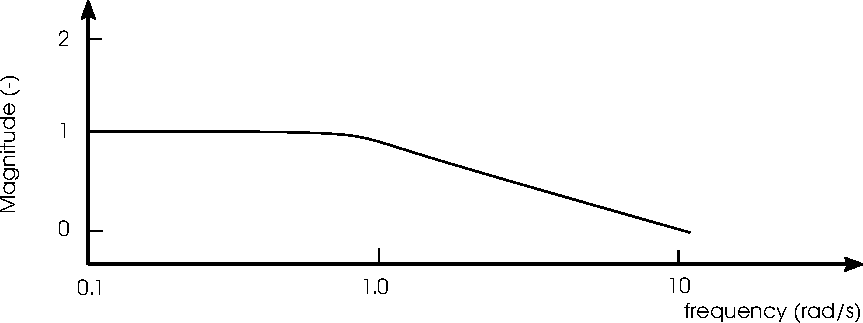
\includegraphics[width=0.75\linewidth]{bode_diagram_open_1.pdf}
	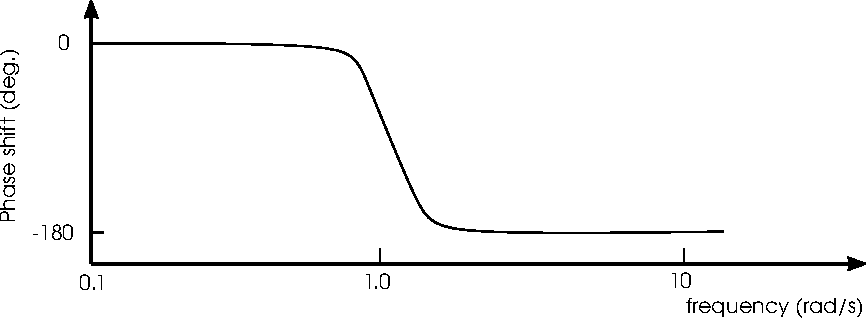
\includegraphics[width=0.75\linewidth]{bode_diagram_open_2.pdf}
	\caption{Approximate Bode diagram based on the setup's open-loop frequency response.}
	\label{fig:approx_bode_diagram_open}
\end{figure}

\mijnfiguur[h!]{width=\linewidth}{wResponse.pdf}{Outcome of the W-shaped response experiment performed using \textit{writeWResponse.m}. The in-flight dead time is approximately $t_d \approx 0.5~s$.}{fig:wResponse}

\mijnfiguur[h!]{width=\linewidth}{blockResponse.pdf}{Outcome of the block-shaped response experiment performed using \textit{writeBlockResponse.m}.}{fig:blockResponse}
 
\mijnfiguur[h!]{width=\linewidth}{tuned_PID1.pdf}{Closed-loop response for a setpoint change from 0~cm to 40~cm, in the abscence of added measurement noise or dead time. $K_P=100;~ K_I=10;~ K_D=0;~K_F=1$. The output of the I controller converges to $\bar{u}$.}{fig:tuned_PID1}
 
\mijnfiguur[h!]{width=\linewidth}{tuned_PID2.pdf}{Closed-loop response for a setpoint change from 20~cm to 40~cm, in the abscence of added measurement noise or dead time. $K_P=1000;~K_I=1;~K_D=100;~K_F=1$.}{fig:tuned_PID2}

\mijnfiguur[h!]{width=\linewidth}{tuned_PID3.pdf}{Closed-loop response for a setpoint change from 20~cm to 40~cm, in the abscence of added measurement noise but with a dead time of $t_d=0.5~s$ on the fan response. $K_P=1000;~ K_I=1;~ K_D=100;~K_F=1$. The closed-loop response has become unstable.}{fig:tuned_PID3}

\mijnfiguur[h!]{width=\linewidth}{tuned_PID4.pdf}{Closed-loop response for a setpoint change from 20~cm to 40~cm, with added measurement noise and subsequent low-pass filtering with time constant $\tau=0.2~s$, and with a dead time of $t_d=0.5~s$ on the fan response. $K_P=50;~ K_I=1;~ K_D=0;~K_F=1$.}{fig:tuned_PID4}

\mijnfiguur[h!]{width=\linewidth}{tuned_PID5.pdf}{Closed-loop dynamics for high proportional gains in the abscence of a setpoint change. $K_P=150;~ K_I=0;~ K_D=0$.}{fig:tuned_PID5}

\mijnfiguur[h!]{width=\linewidth}{tuned_PID6.pdf}{Closed-loop response for a setpoint change from 20~cm to 40~cm at time $t=5~s$, followed by a 7.5~\% decrease in the fan's effectiveness (modeled as a decrease of the parameter $\alpha$ in Eq.~\ref{eq:pingPongModelStates}) at time $t=20~s$. $K_P=80;~ K_I=0;~ K_D=0$.}{fig:tuned_PID6}

\mijnfiguur[h!]{width=\linewidth}{tuned_PID7.pdf}{Closed-loop response for a setpoint change from 20~cm to 40~cm at time $t=5~s$, followed by a 7.5~\% decrease in the fan's effectiveness (modeled as a decrease of the parameter $\alpha$ in Eq.~\ref{eq:pingPongModelStates}) at time $t=20~s$. $K_P=80;~ K_I=10;~ K_D=50;~K_F=1$.}{fig:tuned_PID7}

\mijnfiguur[h!]{width=\linewidth}{ODEModelPID.pdf}{Simulink model \textit{ODEModelPID.slx}. Contains the mathematical model of the setup (Eq.~\ref{eq:pingPongModelStates}) in the subsystem labeled \texttt{system} (Fig.~\ref{fig:ODEModelPID_system}), in closed-loop with a PID controller. The in-flight dead time is added using a \texttt{Transport delay} on the fan's motor response. Noise on the IR proximity sensor's measurement is added using a \texttt{White noise} block, and is subsequently filtered using a low-pass filter.}{fig:ODEModelPID}

\mijnfiguur[h!]{width=\linewidth}{ODEModelPID_system.pdf}{Simulink subsystem \texttt{system} in \textit{ODEModelPID.slx} (Fig.~\ref{fig:ODEModelPID}), containing the implementation of the mathematical model (Eq.~\ref{eq:pingPongModelStates}). Includes saturation of the ball's height between 0~cm and 60~cm.}{fig:ODEModelPID_system}

\mijnfiguur[h!]{width=\linewidth}{ODEModelPID_zdot.pdf}{Simulink subsystem \texttt{zdot} in \textit{ODEModelPID.slx} subsystem \texttt{system} (Fig.~\ref{fig:ODEModelPID_system}), containing the implementation of the derivative of the ball's height $dz/dt = v(t)$ (Eq.~\ref{eq:pingPongModelStates}) with saturation of the height $z(t)$ between 0~cm and 60~cm.}{fig:ODEModelPID_zdot}

\mijnfiguur[h!]{width=\linewidth}{tuned_PID_cohencoon.pdf}{Closed-loop response for a setpoint change from 20~cm to 40~cm, using P, PI, and PID controllers tuned using Cohen and Coon's empirical method (Table~\ref{tab:cohen_coon_tuned1}).}{fig:tuned_PID_cohencoon}

\mijnfiguur[h!]{width=0.78\linewidth}{tuned_PID_zieglernichols_1.pdf}{Closed-loop response for a setpoint change from 20~cm to 40~cm, with a P-controller set to the ultimate control gain of $K_u \approx 114$. The period of the resulting permanent oscillation is equal to $P_u \approx 3.5~s$.}{fig:tuned_PID_zieglernichols_1}

\mijnfiguur[h!]{width=\linewidth}{tuned_PID_zieglernichols_2.pdf}{Closed-loop response for a setpoint change from 20~cm to 40~cm, using P, PI, and PID controllers tuned using Ziegler and Nichols empirical method (Table~\ref{tab:ziegler_nichols_tuned}).}{fig:tuned_PID_zieglernichols_2}

\begin{figure}[t!]
	\centering
	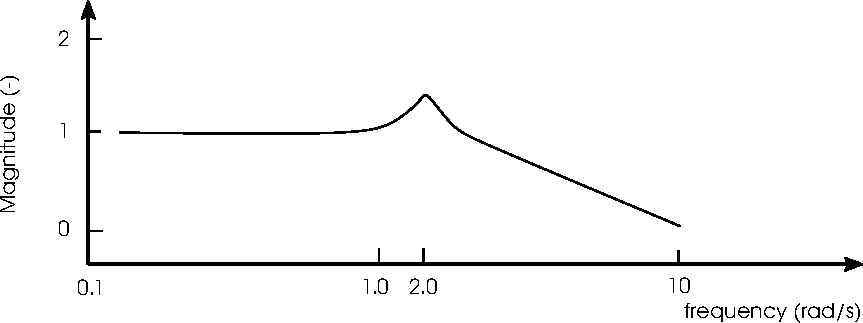
\includegraphics[width=0.75\linewidth]{bode_diagram_closed_1.pdf}
	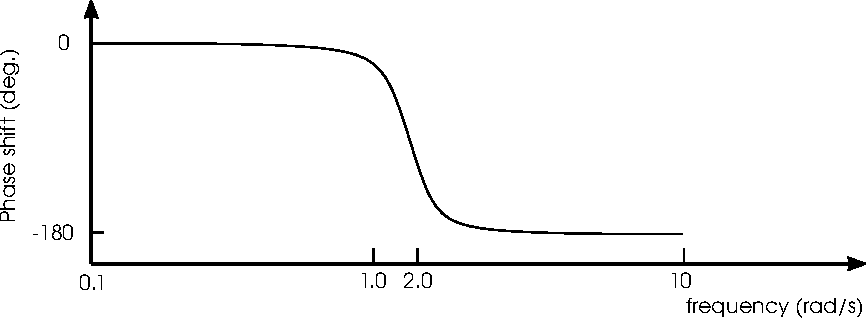
\includegraphics[width=0.75\linewidth]{bode_diagram_closed_2.pdf}
	\caption{Approximate Bode diagram based on the setup's closed-loop frequency response.}
	\label{fig:approx_bode_diagram_closed}
\end{figure}

\mijnfiguur[h!]{width=\linewidth}{tuned_LQR1.pdf}{Closed-loop response for a setpoint change from 20~cm to 40~cm, with a dead time of $t_d=0.5~s$ on the fan's response and in the abscense of measurement noise. Using state feedback with $k_{11} =118$ and $k_{12} =34$.}{fig:tuned_LQR1}

\mijnfiguur[h!]{width=\linewidth}{ODEModelLQR.pdf}{Simulink model \textit{ODEModelLQR.slx}. Contains the mathematical model of the setup (Eq.~\ref{eq:pingPongModelStates}) in the subsystem labeled \texttt{system} (Fig.~\ref{fig:ODEModelPID_system}), in closed-loop with state feedback. Includes a Luenberger state observer to estimate the ball's velocity, which is not measured. The in-flight dead time is added using a \texttt{Transport delay} on the fan's motor response. Noise on the IR proximity sensor's measurement is added using a \texttt{White noise} block, and is subsequently filtered using a low-pass filter.}{fig:ODEModelLQR}

\mijnfiguur[h!]{width=\linewidth}{tuned_LQR2.pdf}{Output of the Luenberger state observer during the closed-loop response for a setpoint change from 20~cm to 40~cm, with a dead time of $t_d=0.5~s$ on the fan's response and in the abscense of measurement noise, and using state feedback with $k_{11} =118$ and $k_{12} =34$ (Fig.~\ref{fig:tuned_LQR1}). For $l_{11} = 995$ and $l_{21}= 245000$, the estimated velocity differed from $v=0~m\cdot s^{\text{-}1}$ when the ball was at rest (prior to the setpoint change), resulting in an unsatisfactory observer design. The result shown here was obtained for $l_{11} = 100$ and $l_{21} = 250000$, and is satisfactory.}{fig:tuned_LQR2}

\end{document}
